\documentclass[en]{../../../eplsummary}
\usepackage{listings}

\usetikzlibrary{calc, trees, positioning, arrows, shapes, shapes.multipart, shadows, matrix, decorations.pathreplacing, decorations.pathmorphing}
\usetikzlibrary{arrows,shapes,snakes,automata,backgrounds,petri}

\hypertitle{cloud-INGI2145}{7}{INGI}{2145}
{Houtain Nicolas, Thibault Gérondal, Kabasele Ndonda Nicolas, Feuillen Gauthier}
{Canini Marco}

\section{Cloud computing}

\subsection{Introduction}

\begin{center}
    \textit{Cloud computing is a model for enabling convenient, 
        on-­demand network access to a shared pool of configurable 
        computing resources (e.g., networks, servers, storage, 
        applications, and services) that can be rapidly provisioned 
        and released with minimal management effort or 
    service provider interaction.}
\end{center}

\begin{tabular}{cm{10cm}}
    \textbf{Cloud commandments (eBay)} &
    \begin{enumerate}
        \item Partition everything
        \item Use asynchony everywhere
        \item Automate everything
        \item Remember that everything fails
        \item Embrace inconsistency
    \end{enumerate}
\end{tabular}

\begin{tabular}{cm{10cm}}
    \textbf{Cloud benefit} &
    \begin{itemize}
        \item Elastic, just-­in-­time infrastructure
        \item More efficient resource utilization
        \item Pay for what you use
        \item Potential to reduce processing time (parallelization)
        \item Leverage multiple data centers (high availability)
    \end{itemize}
\end{tabular}


\subsubsection{Hardware scalability}

Cloud need for \textbf{scalability} because modern application require
huge amounts of processing and data. Cluster (\textit{room-sized}) and datacenter 
(\textit{building-sized}) can provide the resources needed.
They are composed of \textbf{rack} which is a aggregation of storage devices, many
nodes and switch to connect nodes together. Unfortunately, they are not perfect.
\begin{enumerate}
    \item Difficult to dimension because they must be provisioning for the peak load
    \item Expensive in hardware invest, expertise (ex: special software) and maintenance
    \item Difficult to scale because adding new machines is not easy
\end{enumerate}


\subsubsection{Model}
Cloud computing is a business models where everything is a service:
\begin{itemize}
    \item \textbf{SaaS}: Software as a service, soft. run on distant server 
        instead on running on the user machine.
    \item \textbf{PaaS}: Platform as a service.  Customers handle the application.
    \item \textbf{IaaS}: Infrastructure as a service. Customers handle the 
        middleware and application. Provider handle hardware.
\end{itemize}

\subsubsection{Types}
There also have three types of cloud : 
\begin{itemize}
    \item \textbf{Public}: commercial commercial service open to almost anyone.
    \item \textbf{Community}: shared by several similar organization
    \item \textbf{Private}: shared within a organization
\end{itemize}
In this course we focus on public cloud.

\subsubsection{Applications}

Typically, applications that involve large amounts of computation, storage,
bandwidth Especially when lots of resources are needed quickly or load varies
rapidly.

\begin{itemize}
    \item \textbf{Web app}: Near the edge of the application focus is on vast 
        numbers of clients and rapid response
    \item \textbf{Processing pipelines}: Inside we find data-­intensive services that 
        operate in a pipelined manner, asynchronously
    \item \textbf{Batch processing}: Deep inside the application we see a world of 
        virtual computer clusters that are scheduled to 
        share resources and on which applications like 
        MapReduce (Hadoop) are very popular
\end{itemize}


\subsubsection{Virtualization}
It is used to simulate multiple physical machine for the consumer with different
capabilities. It's powerful for security and isolation because VM cannot influence
other and it provides high flexibility. In the other hand, performance is hard 
to predict because other VM run on the same physical machine.

\subsubsection{Challenge}
\begin{tabular}{m{0.5\linewidth}m{0.5\linewidth}}
    \begin{itemize}
        \item Availability
        \item Data lock-in (moving data)
        \item Data confidentiality and auditability 
        \item Data transfer bottlenecks
        \item Performance unpredictability for VM
    \end{itemize}
    &
    \begin{itemize}
        \item Scalable storage
        \item Bugs in large distributed systems
        \item Scaling quickly
        \item Reputation fate sharing
        \item Software licensing
    \end{itemize}
\end{tabular}



\section{Design for scale}

A system is scalable if it can easily adapt to 
increased (or reduced) demand. Scalablity
is usually limited by some sort of bottleneck.

\subsection{Parallelism programming}

\subsubsection{Vocabulary}
\begin{description}
    \item[Parallelism]: refers to techniques to make programs faster by
        performing several computations in parallel.

    \item[Concurrency]: is the composition of independently executing
        computations.

\end{description}

\subsubsection{Parallelization}
\begin{itemize}
    \item \textbf{Amdahl's law}:

        \begin{tabular}{m{0.5\linewidth}m{0.5\linewidth}}
            $$\quad S = \frac{1}{\alpha +
            \frac{1-\alpha}{N}}$$ where $\alpha$ is the sequential part and $N$ the
            number of cores.
            &
            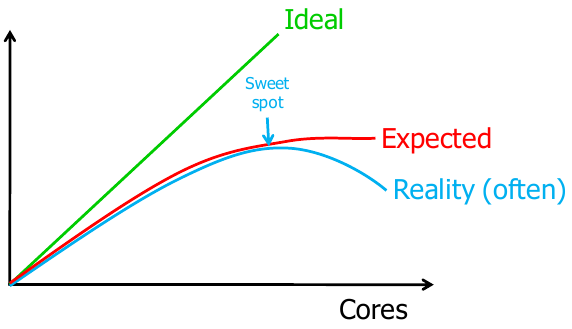
\includegraphics[width=6cm]{img/amdahl.png}
        \end{tabular}

        The coarse-grain (low rate communication) opposed to fine-grain (high rate) 
        parallelism is more efficient because it limits the communication and 
        coordination overheads by allow bigger task.

    \item \textbf{Dependencies}: Some task need to be after other which limits the degree of 
        parallelism. $\rightarrow$ Scheduling problem
\end{itemize}

\subsubsection{Synchronization}
Synchronization is needed when state is updated by different entities
(threads,process,servers,...)
\begin{description}
    \item[Race condition]: Result of the computation depends on the exact
        timing of the two threads of execution,i.e, the order in which instruction 
        are executed.

\end{description}

\subsubsection{Architecture}
\begin{itemize}
    \item Symmetric multiprocessing (SMP): all processors share same memory.

        \begin{tabular}{m{0.7\linewidth}m{0.3\linewidth}}
            \begin{itemize} 
                \item[+] Simplicity and easy to load balance 
                \item[-] Scalability limited and expensive
            \end{itemize}
            &
            \begin{tiny}
                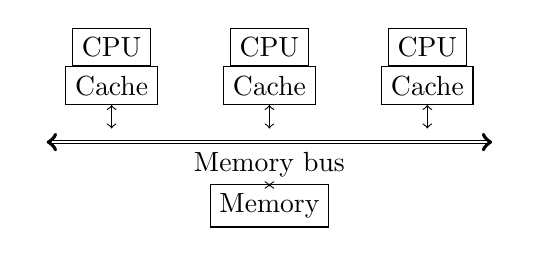
\begin{tikzpicture}
                    \node[draw, rectangle] (1) {CPU};
                    \node[draw, rectangle] (2) [right=of 1] {CPU};
                    \node[draw, rectangle] (3) [right=of 2] {CPU};

                    \node[draw, rectangle] (11) [below=0cm of 1] {Cache};
                    \node[draw, rectangle] (21) [below=0cm of 2] {Cache};
                    \node[draw, rectangle] (31) [below=0cm of 3] {Cache};

                    \node (12) [below=0.3cm of 11] {};
                    \node (22) [below=0.3cm of 21] {};
                    \node (32) [below=0.3cm of 31] {};

                    \node (tmp) [below left= -0.2cm and 0.7cm of 12] {};
                    \node (tmp2) [below right=-0.2cm and 0.7cm of 32] {};

                    \draw (tmp) edge[double, <->] node[below](p) {Memory bus} (tmp2);
                    \draw (12) edge[<->] (11);
                    \draw (22) edge[<->] (21);
                    \draw (32) edge[<->] (31);

                    \node[draw, rectangle] (mem) [below=1.0cm of 21] {Memory};
                    \draw (mem) edge[<->] (p);
                \end{tikzpicture}
            \end{tiny}
        \end{tabular}

    \item Non Uniform memory architecture (NUMA)

        \begin{tabular}{m{0.7\linewidth}m{0.3\linewidth}}
            \begin{itemize} 
                \item[+] Better scalability and faster memory
                \item[-] Complicates programming and scalability limited
            \end{itemize}
            &
            \begin{tiny}
                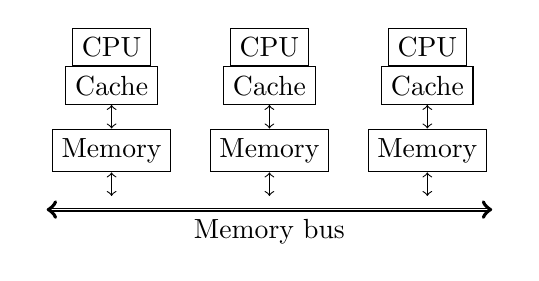
\begin{tikzpicture}
                    \node[draw, rectangle] (1) {CPU};
                    \node[draw, rectangle] (2) [right=of 1] {CPU};
                    \node[draw, rectangle] (3) [right=of 2] {CPU};

                    \node[draw, rectangle] (11) [below=0cm of 1] {Cache};
                    \node[draw, rectangle] (21) [below=0cm of 2] {Cache};
                    \node[draw, rectangle] (31) [below=0cm of 3] {Cache};

                    \node[draw, rectangle] (12) [below=0.3cm of 11] {Memory};
                    \node[draw, rectangle] (22) [below=0.3cm of 21] {Memory};
                    \node[draw, rectangle] (32) [below=0.3cm of 31] {Memory};

                    \node (13) [below=0.3cm of 12] {};
                    \node (23) [below=0.3cm of 22] {};
                    \node (33) [below=0.3cm of 32] {};

                    \node (tmp) [below left= -0.2cm and 0.7cm of 13] {};
                    \node (tmp2) [below right=-0.2cm and 0.7cm of 33] {};

                    \draw (tmp) edge[double, <->] node[below](p) {Memory bus} (tmp2);
                    \draw (12) edge[<->] (11);
                    \draw (22) edge[<->] (21);
                    \draw (32) edge[<->] (31);

                    \draw (12) edge[<->] (13);
                    \draw (22) edge[<->] (23);
                    \draw (32) edge[<->] (33);
                \end{tikzpicture}
            \end{tiny}
        \end{tabular}

    \item Shared Nothing

        \begin{tabular}{m{0.7\linewidth}m{0.3\linewidth}}
            \begin{itemize} 
                \item[+] Nice scalability
                \item[-] Requires different programming model
            \end{itemize}
            &

            \begin{tiny}
                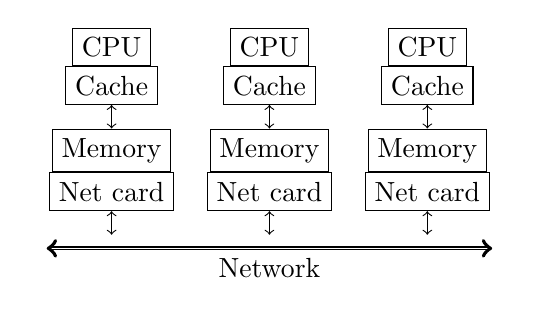
\begin{tikzpicture}
                    \node[draw, rectangle] (1) {CPU};
                    \node[draw, rectangle] (2) [right=of 1] {CPU};
                    \node[draw, rectangle] (3) [right=of 2] {CPU};

                    \node[draw, rectangle] (11) [below=0cm of 1] {Cache};
                    \node[draw, rectangle] (21) [below=0cm of 2] {Cache};
                    \node[draw, rectangle] (31) [below=0cm of 3] {Cache};

                    \node[draw, rectangle] (12) [below=0.3cm of 11] {Memory};
                    \node[draw, rectangle] (22) [below=0.3cm of 21] {Memory};
                    \node[draw, rectangle] (32) [below=0.3cm of 31] {Memory};

                    \node[draw, rectangle] (14) [below=0cm of 12] {Net card};
                    \node[draw, rectangle] (24) [below=0cm of 22] {Net card};
                    \node[draw, rectangle] (34) [below=0cm of 32] {Net card};

                    \node (13) [below=0.3cm of 14] {};
                    \node (23) [below=0.3cm of 24] {};
                    \node (33) [below=0.3cm of 34] {};

                    \node (tmp) [below left= -0.2cm and 0.7cm of 13] {};
                    \node (tmp2) [below right=-0.2cm and 0.7cm of 33] {};

                    \draw (tmp) edge[double, <->] node[below](p) {Network} (tmp2);
                    \draw (12) edge[<->] (11);
                    \draw (22) edge[<->] (21);
                    \draw (32) edge[<->] (31);

                    \draw (13) edge[<->] (14);
                    \draw (23) edge[<->] (24);
                    \draw (33) edge[<->] (34);
                \end{tikzpicture}
            \end{tiny}
        \end{tabular}

\end{itemize}


\subsection{Distributed programming}

\subsubsection{Vocabulary}
\begin{description}
    \item[Faults]: Some component is not working correctly
    \item[Failure]: System as a whole is not working correctly
\end{description}

\subsubsection{Wide-area network}
The transfert speed for some data are defined by some attributs:
\begin{enumerate}
    \item Propagation delay
    \item Bottlenecks capacity on the path
    \item Queueing delay, loss, reordering, congestion, rtt 
        (take in account by TCP)
\end{enumerate}

$\rightarrow$ wide-area networks complicates the communication and faults are
more common

\subsubsection{Faults}

Fault are a common event in distributed system and some faults
are correlated.

\begin{itemize}
    \item \textbf{Crash faults}: node simply stop
    \item \textbf{Rational behavior}: owner manipulates node to increase profit
        (ex: lies on the routes to have traffic through it's own AS)
    \item \textbf{Byzantine faults}: faulty node could do anything (ex: stop, send spam,
        attack other, tell lies,...)
\end{itemize}

To prevent fault, we can \textit{prevent} them by using verification,
\textit{detect} them or \textit{mask} them by using replicas. The problem of
using \textbf{replicas} is to be able to maintain consistency between them!

\subsubsection{Consistency}

\begin{itemize}
    \item \textbf{Strong consistency}: After update completes, all subsequent
        accesses will return the updated value

    \item \textbf{Weak consistency}: After update completes, accesses do not
        necessarily return the updated value;; some condition must be satisfied
        first (such as update needs to reach all the replicas)

    \item \textbf{Eventual consistency}: Specific form of weak consistency: If no
        more updates are made to an object, then eventually all reads will return
        the latest value

    \item \textbf{Causal consistency}: If client A has communicated to client B that it
        has updated a data item, a subsequent access by B will return the updated
        value, and a write is guaranteed to supersede the earlier write. Client C
        that has no causal relationship to client A is subject to the normal
        eventual consistency rules

    \item \textbf{Read-your-writes consistency}: Client A, after it has updated a data
        item, always accesses the updated value and will never see an older
        value.

    \item \textbf{Session consistency}: Like previous case but in the context of a
        session, for as long as the sessions remains alive.

    \item \textbf{Monotonic read consistency}: If client A has has seen a particular value
        for the object, any subsequent accesses will never return any previous
        values

    \item \textbf{Monotonic write consistency}: In this case the system guarantees to
        serialize the writes by the same process
\end{itemize}

We can combine them, and monotonic reads + read-your-write are most desirable
than eventual consistency.

\paragraph{Storage system consistency: example}

We have N nodes that can store data.
To write a value: Pick W replicas and write the value to each, using a fresh timestamp
To read a value:
\begin{itemize}
    \item Pick R replicas and read the value from each
    \item Return the value with the highest timestamp
    \item If any replicas had a lower timestamp, send them the newer value
\end{itemize}

Strong consistency :
\begin{description}
    \item[Majority quorum] Always write to and read from a majority of nodes. At least one node knows the most recent value. tolerate up to ⌈N/2⌉ - 1 crashes. But have to read/write ⌊N/2⌋ + 1 values.
    \item[Read/write quorums] Read R nodes, write W nodes, s.t. R + W > N. Adjust performance of reads/writes. But availability can suffer.

        \begin{tabular}{m{5cm}m{12cm}}
            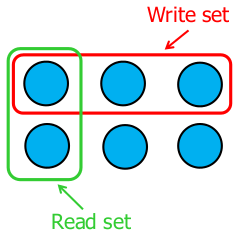
\includegraphics[width=3cm]{img/replicas} &
            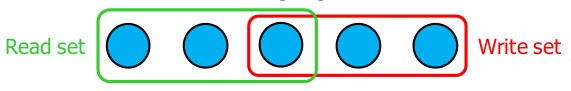
\includegraphics[width=7cm]{img/replicas2}
            \begin{itemize}
                \item[$\rightarrow$] Strong consistency
            \end{itemize} \\
        \end{tabular}
    \item[Consensus solutions] Paxos (for crash faults), PBFT (for Byzantine faults). Idea : Correct replicas ``outvote'' faulty ones.
\end{description}

The cap theorem : We can get at most two out of the three
\begin{itemize}
    \item Consistency : All clients single up-to-data copy of the data, even in the presence of concurrent updates
    \item Availability: Every request (including updates) received by a non-failing node in the system must result in a response, even when faults occur
    \item Partition-tolerance: Consistency and availability hold even when the network partitions
\end{itemize}

Dealing with network partitions when a partition is cut : Enter an explicit partition mode that can limit some operations.


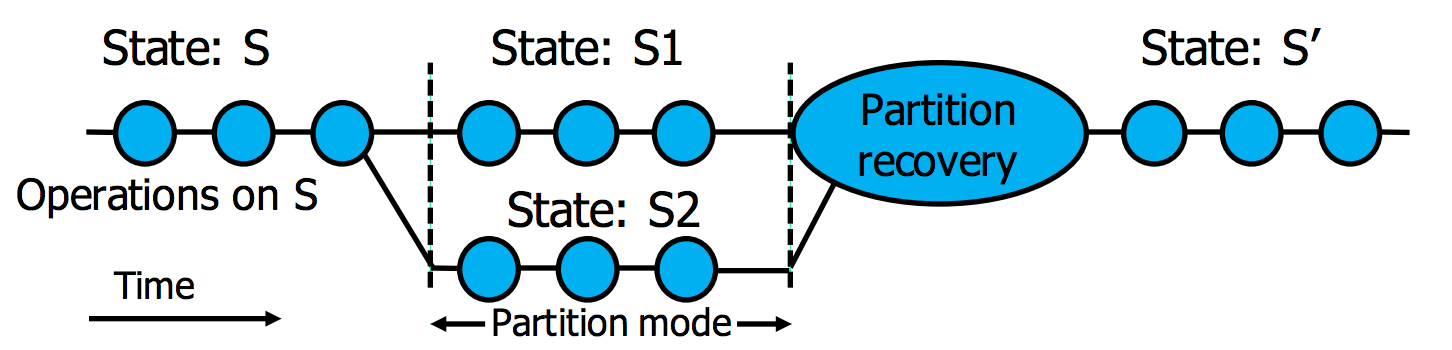
\includegraphics[width=\linewidth]{img/part}




\paragraph{Consensus}
\begin{enumerate}
    \item Clients send requests to each of the replicas
    \item Replicas coordinate and each return a result
    \item Client chooses one of the results, e.g., the one that is 
        returned by the largest number of replicas
    \item If a small fraction of the replicas returns the wrong result, or 
        no result at all, they are 'outvoted' by the other replicas
\end{enumerate}


\subsubsection{CAP theorem}
\begin{center}
    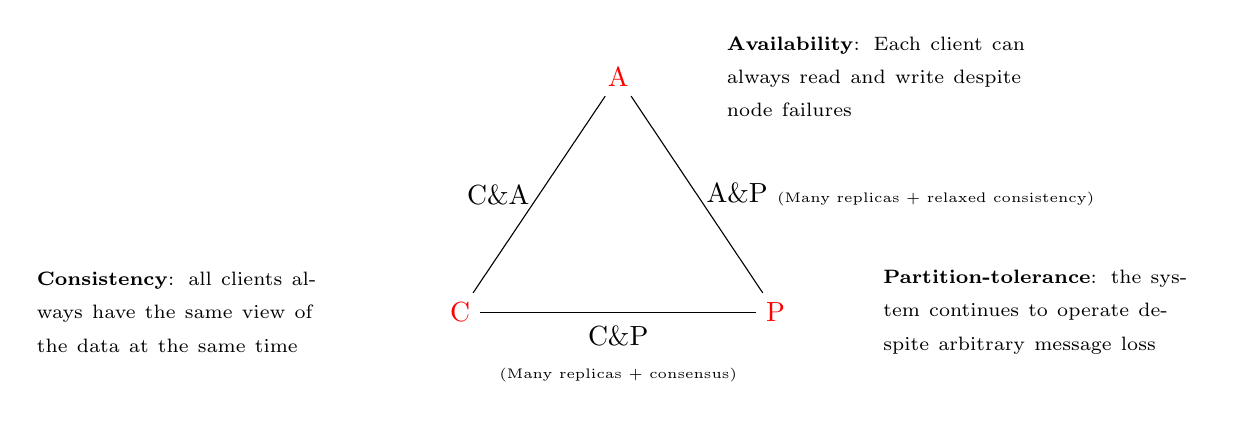
\begin{tikzpicture}
        \node (A) {\textcolor{red}{A}};
        \node (C) [below left= 2.5cm and 1.5cm of A] {\textcolor{red}{C}};
        \node (P) [below right= 2.5cm and 1.5cm of A] {\textcolor{red}{P}};

        \node[right =1cm of A, text width=4cm] {\scriptsize \textbf{Availability}: Each client can always read
        and write despite node failures};

        \node[left =1cm of C, text width=4cm] {\scriptsize \textbf{Consistency}: all clients always have the
        same view of the data at the same time};

        \node[right =1cm of P, text width=4cm] {\scriptsize \textbf{Partition-tolerance}: the
        system continues to operate despite arbitrary message loss};

        \draw (A) edge[-] node[left] {C\&A} (C);
        \draw (A) edge[-] node[right] {A\&P \tiny (Many replicas + relaxed consistency)} (P);
    \draw (C) edge[-] node[below] {\begin{tabular}{c}C\&P\\ \tiny (Many replicas + consensus) \end{tabular}} (P);
    \end{tikzpicture}
\end{center}


\paragraph{Actually}, we have a lot of partition and we have a trade-off
between C and A. \textbf{ACID} (atomicity, consistency, isolation, durability)
become \textbf{BASE} (basically available, soft-state, eventually consistent).


\subsection{Structure}
\begin{figure}[!h]
    \centering
    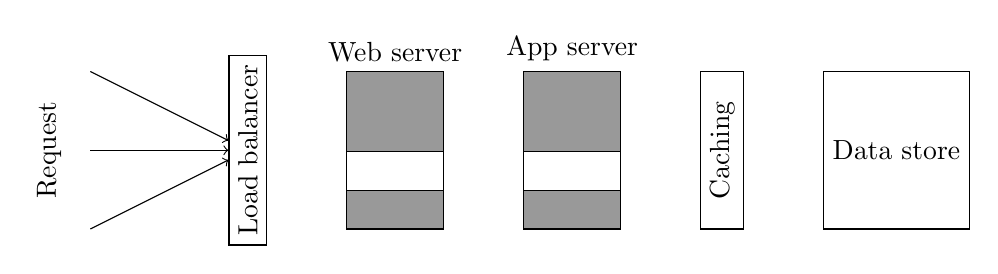
\begin{tikzpicture}

        \node[draw, rectangle, minimum height= 2cm] (L) {\rotatebox{90}{Load balancer}};
        \node[draw, rectangle, fill=black!40, minimum height= 2cm, text width=1cm, right= of L] (W) {};
        \node[draw, rectangle, fill= white, minimum height= 0.5cm, text width=1cm, below=-1cm of W] (W1) {};
        \node[above=0cm of W] (1) {Web server};

        \node[draw, rectangle, fill=black!40, minimum height= 2cm, text width=1cm, right= of W] (A) {};
        \node[draw, rectangle, fill=white, minimum height= 0.5cm, text width=1cm, below=-1cm of A] (A1) {};
        \node[above=0cm of A] (1) {App server};

        \node[draw, rectangle, minimum height= 2cm, right= of A] (C) {\rotatebox{90}{Caching}};
        \node[draw, rectangle, minimum height= 2cm, right= of C] (D) {Data store};

        \draw[->] (-2, 0) -- (L);
        \draw[->] (-2, -1) -- (L);
        \draw[->] (-2, 1) -- (L);

        \node[left=2cm of L] (R) {\rotatebox{90}{Request}};

    \end{tikzpicture}
    \caption{Cloud structure with 
        caching which is central to responsiveness. Cached data are used by the inner
    services to shield them form online load}
\end{figure}

\begin{itemize}
    \item \textbf{Stateless server}: Views a client request as an independent 
        transaction and responds to it


        Easy to scale and more robust because instance failure does not require
        overheas restoring state

    \item \textbf{Statefull server}: Scaling is challenging because we need to maintains 
        the state.

        \paragraph{Traditionnal approach is replication}:

        \begin{tabular}{m{12cm}m{5cm}}
            \begin{itemize}
                \item Data is written to a \textit{master server} and then
                    replicated to one or more \textit{slave servers}
                    (synchronously or asynchronously)
                \item Read operations can be handled by the slaves
            \end{itemize}
            But in this case, master becomes the write bottleneck and single point of failure.
            &
            \centering
            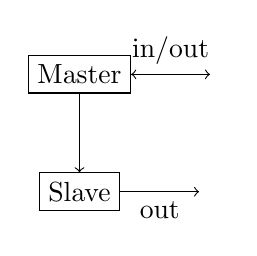
\begin{tikzpicture}
                \node[draw, rectangle] (M) {Master};
                \node[draw, rectangle, below=1cm of M] (S) {Slave};
                \node (I) [right= of M] {};
                \node (O) [right= of S] {};

                \draw[->, double] (I) edge node[above] {in/out} (M);
                \draw[<-, double] (I) edge (M);
                \draw[<-, double] (O) edge node[below] {out}(S);
                \draw[->, double] (M) edge (S);
            \end{tikzpicture}
        \end{tabular}


        \paragraph{Sharding with partitionning}
        The idea is to split data between multiple 
        machines and have a way to make sure that
        the data is available on the right place.
        Typically, define a \textbf{sharding key} and create a \textbf{shard mapping}.

        \begin{tabular}{cm{10cm}}
            This allow to have &
            \begin{itemize}
                \item a really high availability
                \item increase read and write throughput
                \item the possibility 
                    of doing more work in parallel within the application server.
                \item[But] the challenge is to find a good partitionning scheme.
            \end{itemize}
        \end{tabular}

        \textbf{Sharding} is not only for partitioning data 
        within a database, but can also be use to partition data across caching 
        servers (memcached, redis).
\end{itemize}

\paragraph{First-tier parallelism}
Parallelism is vital for fast interactive services, and 
parallel actions must focus on the \textbf{critical path}. This is the
contributor delay for the response delay and do
not care about asynchronous that are shortly.

\begin{center}
    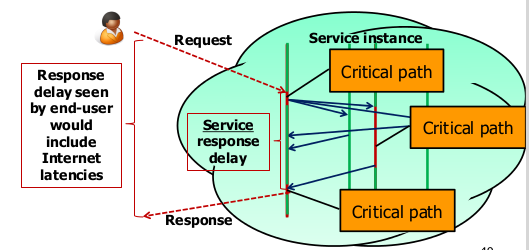
\includegraphics[width=9cm]{img/critical}
\end{center}


Note that update for replicas are typically done in asynchronous way, so we
might not experience much delay on the critical path.

$\rightarrow$ Asynchronous operations decouple systems and 
enable quicker responses at the expense strong 
consistency.
Indeed, this can rise some issues which result in inconsistency:
\begin{itemize}
    \item We don't know in which order replicas applying the update
    \item The leader can crash before replicas change and lose some
        update
\end{itemize}


\section{Cloud storage}

\begin{center}
    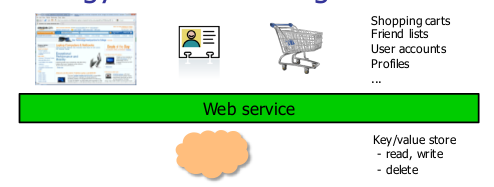
\includegraphics[width=12cm]{img/storage}
\end{center}

Many cloud services have a similar structure, 
But the actual storage service is very simple (Read/write 'blocks',
similar to a giant hard disk) and the translation done by the web service.

\paragraph{Ideal store}
\begin{itemize}
    \item Perfect durability – nothing would ever disappear in a crash
    \item 100\% availability – we could always get to the service
    \item Zero latency from anywhere on earth – no delays!
    \item Minimal bandwidth utilization – we only send across the network what we absolutely need
    \item Isolation under concurrent updates – make sure data stays consistent
\end{itemize}

BUT the “cloud” exists over a physical network (communication take time + limited bandwith)
and The “cloud” has imperfect hardware (failures)

\paragraph{Observation}
\begin{itemize}
    \item Read-­only (or read-­mostly) data is easiest to support
    \item Granularity matters: “Few large-­object” tasks generally 
        tolerate longer latencies than “many small-­object” tasks


        But it’s much more expensive to replicate or to update!

    \item[$\rightarrow$] Maybe it makes sense to develop separate solutions for large 
        read-­mostly objects vs. small read-­write objects!
        Different requirements $\rightarrow$ different technical solutions
\end{itemize}


\subsection{Key-value stores (KVS)}
The key-­value store (KVS) is a simple 
abstraction for managing persistent state where data is 
organized as (key,value) pairs with three basic operation:
\begin{enumerate}
    \item \texttt{PUT(key, value)}
    \item \texttt{value = GET(key)}
    \item \texttt{DEL(key)}
\end{enumerate}

\paragraph{Concurrency control}
Most systems use locks on individual items.



\subsubsection{Amazon dynamo}
\begin{figure}[!h]
    \centering
    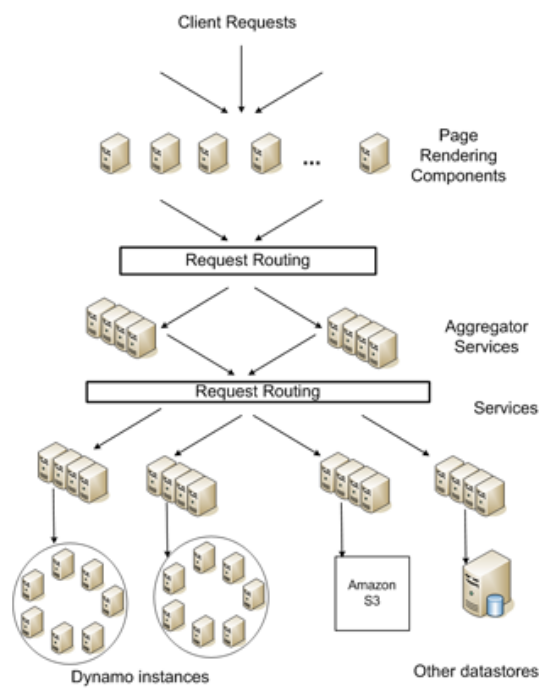
\includegraphics[width=5cm]{img/AWSplat}
    \caption{Amazon dynamo. 
        AWS is \textbf{Availability\&Partition-tolerance} and follow 
    \textbf{BASE} philosophy.}
\end{figure}

\begin{tabular}{cm{10cm}}
    Dynamo is :&
    \begin{itemize}
        \item High performance with low latency
        \item High scalable
        \item High available key storage, especially for writes
        \item Partition/fault-tolerant
        \item Eventually consistent (sacrify for high availability)
    \end{itemize}
\end{tabular}
Very low latency writes, reconciliation in reads (last write wins). Object stored are 
relatively small (typically <1MB)

\paragraph{Key Techniques}
\begin{itemize}
    \item \textbf{Consistent hashing}: dynamically partitions a set of keys
        over a set of storage nodes (hash keys and give 
        a key of m-bits). One key range per virtual node.

        \paragraph{Data partitioning and load balancing}
        A key is assigned to the closest successor node id 
        (key $k$ is assigned to the first node with $id \geq k$)

        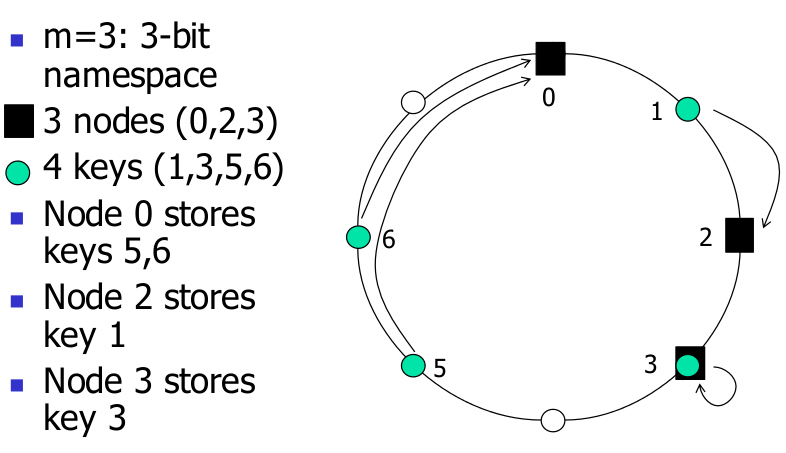
\includegraphics[width=5cm]{img/consistent}

        \begin{center}
            Each node has at most $(1+\epsilon) \frac{K}{N}$ keys with $N$ nodes, $K$ keys
            and $\epsilon=O(log(N))$  To leverage heterogeneity between node ($\neq$ processing
            capabilities), Dynamo uses virtual nodes. Physical are responsible for one or more 
            virtual node depending of its capability.
            %TODO: why epsilon=0 with virtual nodes?
        \end{center}

        \paragraph{Replication}
        Replication is done on the successors node because if the node fail, it's the successor
        which will take failed node keys.

        \begin{center}
            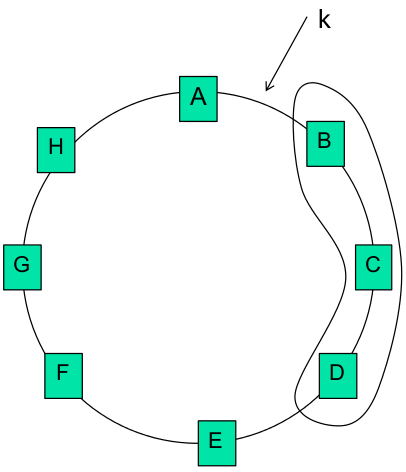
\includegraphics[width=5cm]{img/dynamoReplica}
        \end{center}

        Replication is may in asynchronous way (eventual consistency), and
        key data versioning technique is done with vector clocks.


        If the replica A in the preference list is down then
        another replica is created on a new node.
        In this case, coordinator will involve D that substitutes
        A until A comes back again. When D gets info A is
        back up it hands back the data to A


    \item \textbf{Vector clocks}: Each write to a key k is associated with a 
        vector clock VC(k) which is an array (map) of integers (one entry VC(k)[i] for each node i).

        This is use for tracking causal dependencies among different versions 
        of the same key (data)

        \begin{center}
            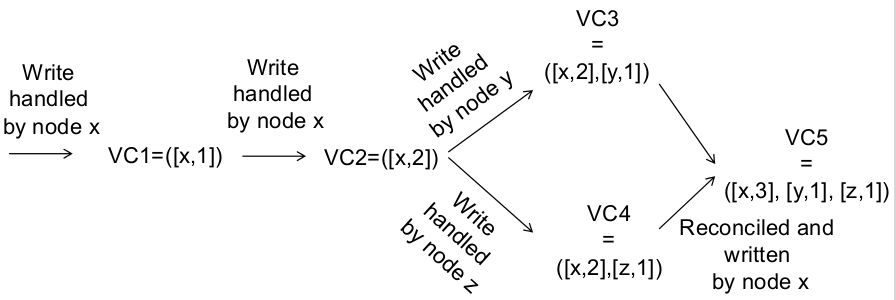
\includegraphics[width=5cm]{img/vectorClock}
        \end{center}

    \item \textbf{Sloppy quorums}: In order to enforce consistency, to response
        to a read or write operation the node must asl to a \textit{quorum}
        which is the minimum number of votes that a distributed transaction has
        to obtain.

        \begin{itemize}
            \item $R$ number of nodes that participate in a get, $W$ number
                of node that participate in a write and $R+W > N$

            \item \textbf{Put}: Generate new $VC$, write locally, send value $VC$
                to N selected nodes from preference list and wait for $W-1$

            \item \textbf{Get}: Send read to $N$ selected nodes from preference list, 
                wait for $R$, select highest versions per $VC$ and return
                all such versions. 

                Writeback merge versions.

            \item[Note]
                \begin{enumerate}
                    \item Note that each node has routing info to all other node
                        to reduce latency (but this is less scalable)
                \end{enumerate}
                To handle puts and gets, 3 differents ways:
                \begin{itemize}
				\item \textbf{Extended preference list} N nodes from preference list +
				some additional nodes (following the circle) to account for failure.
				\item \textbf{Failure-free case} Node from preference list are involved
				in get/put
				\item \textbf{Failures} First N alive nodes from extended preference list
				are involved.
			\end{itemize}
        \end{itemize}

        \textbf{Sloppy} allow availability under a much wider range of 
        partitions (failures) but sacrifice consistency. The
        N selected nodes are the first N healthy 
        nodes.

    \item \textbf{Anti-entropy protocol using hash/merkle tree}:
        Each Dynamo node keeps a Merkle tree for 
        each of its key ranges. Hash trees can be used to verify any kind of data stored.

        \begin{center}
            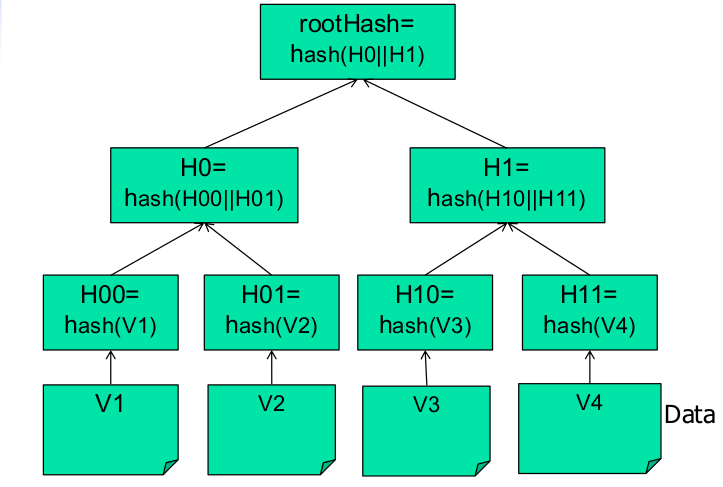
\includegraphics[width=5cm]{img/merkle}
        \end{center}

        Compares the root of the tree with replicas
        \begin{itemize}
            \item If equal, all keys in a range are equal (replicas in sync)
            \item If not equal 
                Traverse the branches of the tree to pinpoint the children that differ
                The process continues to all leaves
                Synchronize on those keys that differ
        \end{itemize}

    \item \textbf{Gossip-based group membership protocol}: 


        Membership info are also eventually 
        consistent — propagated by background 
        gossip protocol.
        \begin{itemize}
            \item Node contacts a random node every 1s
            \item 2 nodes reconcile the membership info and partitioning/placement
                metadata
        \end{itemize}


        \paragraph{Unreliable failure detection (FD)}
        Used to refresh the healthy node info in the extended 
        preference list. In the presence of steady rate of client request
        \begin{enumerate}
        	\item Node A may consider node B failed if node B
        		  does not respond to A's message
		\item Node A then uses an alternates nodes to services 
		requests that maps to B partitions
		\item A periodically checks on B
        \end{enumerate}
        If there s no client requests to drive traffic between two nodes,
        nodes are unaware whether the other has crashed or not
        \footnote{http://www.allthingsdistributed.com/2007/10/amazons\_dynamo.html}.
\end{itemize}


\section{MapReduce}

\begin{figure}[!h]
    \centering
    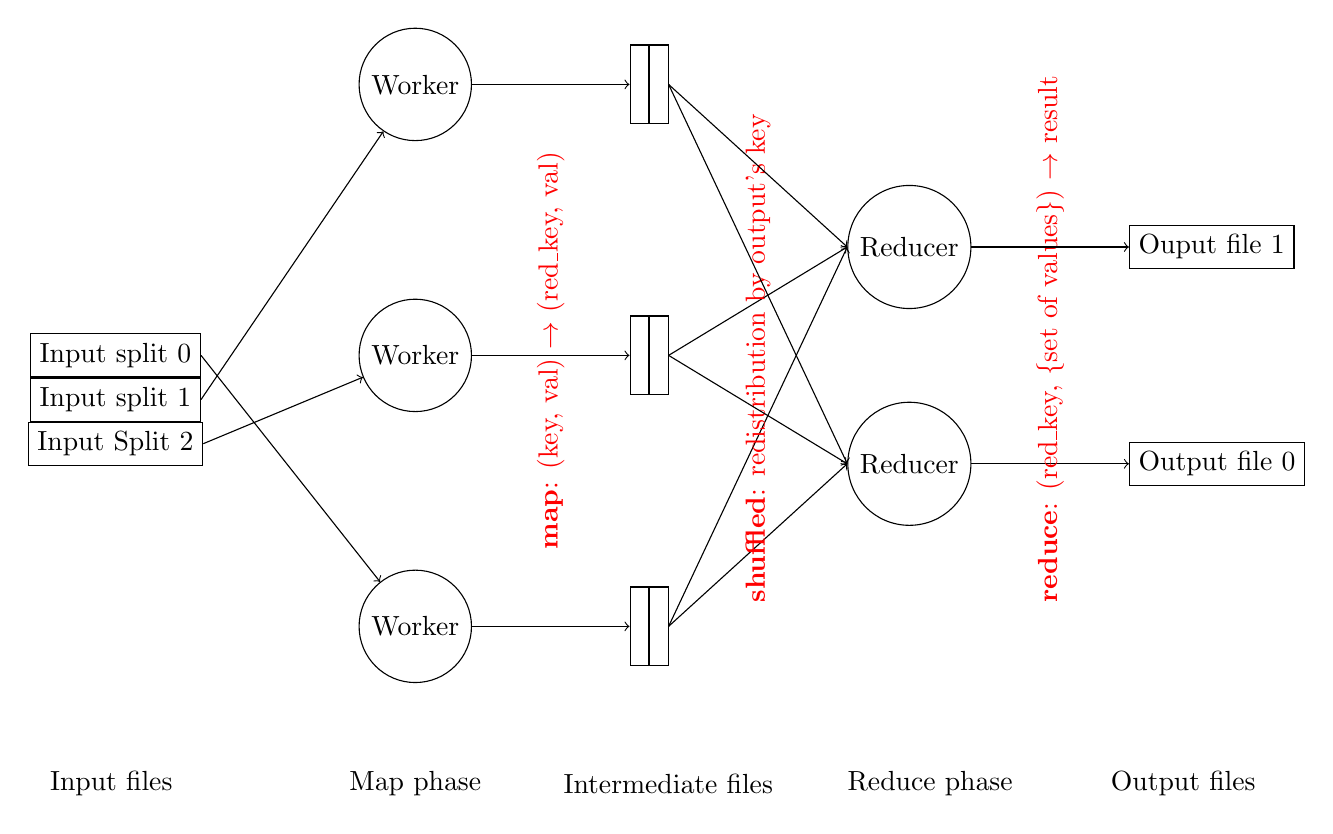
\begin{tikzpicture}[node distance=2cm]
        \node[draw, rectangle] (I0) {Input split 0};
        \node[draw, rectangle, below=0cm of I0] (I1) {Input split 1};
        \node[draw, rectangle, below=0cm of I1] (I2) {Input Split 2};

        \node[draw, circle, right=of I0 ] (W2) {Worker};
        \node[draw, circle, below=of W2 ] (W1) {Worker};
        \node[draw, circle, above=of W2 ] (W3) {Worker};

        \node[draw, minimum height=1cm,rectangle, right=of W1 ] (F1) {};
        \node[draw, minimum height=1cm, rectangle, right=of W2 ] (F2) {};
        \node[draw, minimum height=1cm, rectangle, right=of W3 ] (F3) {};

        \node[draw, rectangle, minimum height=1cm, right=0cm of F1 ] (FF1) {};
        \node[draw, rectangle, minimum height=1cm,right=0cm of F2 ] (FF2) {};
        \node[draw, rectangle, minimum height=1cm, right=0cm of F3 ] (FF3) {};

        \node[draw, circle, above right=1cm and 2.5cm of FF1 ] (R1) {Reducer};
        \node[draw, circle, below right=1cm and 2.5cm of FF3 ] (R2) {Reducer};

        \node[draw, rectangle, right=of R1 ] (O1) {Output file 0};
        \node[draw, rectangle, right=of R2 ] (O2) {Ouput file 1};

        \draw (I0.0) edge[->](W1);
        \draw (I1.0) edge[ ->](W3);
        \draw (I2.0) edge[ ->](W2);

        \draw (W1.0) edge[->] (F1.180);
        \draw (W2.0) edge[->] node 
        {\rotatebox{90}{ \textcolor{red}{\textbf{map}: (key, val) $\rightarrow$ (red\_key, val)}}} (F2.180);
        \draw (W3.0) edge[->] (F3.180);

        \draw (FF1.0) edge[->] (R1.180);
        \draw (FF1.0) edge[->] (R2.180);
        \draw (FF2.0) edge[->] node[below=-2.5cm]
        {\rotatebox{90}{ \textcolor{red}{\textbf{shuffled}: redistribution by output's key}}} (R2.180);
        \draw (FF2.0) edge[->] (R1.180);
        \draw (FF3.0) edge[->] (R1.180);
        \draw (FF3.0) edge[->] (R2.180);

        \draw (R1.0) edge[->] node[above=-2cm]
        {\rotatebox{90}{ \textcolor{red}{\textbf{reduce}: (red\_key, \{set of values\}) $\rightarrow$ result}}} (O1.180); 
        \draw (R2.0) edge[->] (O2.180);

        \node[below=1cm of W1] (2) {Map phase};
        \node[left=of 2] (1) {Input files};
        \node[right=0.8cm of 2] (3){Intermediate files};
        \node[right=0.7cm of 3] (4){Reduce phase};
        \node[right=1cm of 4] (5){Output files};


    \end{tikzpicture}

    \centering
    \begin{itemize}
        \item \textbf{File system} distributed across all nodes with replication
        \item \textbf{Driver program} on the master to keeping all node busy
        \item \textbf{Runtime system} which control nodes
    \end{itemize}
    \caption{MapReduce where mapper and reducer should be \textbf{stateless}
    }
\end{figure}


A variety of different tasks can be expressed 
as a single-­pass MapReduce program which are specifically designed
for \textbf{batch operation} over large amounts of data:
\begin{itemize}
    \item filter, collect, aggregate, join on shared element
\end{itemize}

\paragraph{Not for MapReduce}
\begin{itemize}
    \item sorting don't work 
    \item algorithms that depend on shared global state during 
        processing are difficult to implement.
    \item Process live data at high throughput and low latency

\end{itemize}


\subsection{Failure}
On worker crash we rely on the file system being shared 
across all the nodes. 
\begin{itemize}
    \item If the node wrote its output and then crashed, 
        the file system is likely to have a copy of the complete output.
    \item If the node crashed before finishing its output, the master 
        see that the job isn’t making progress, and restarts the 
        job elsewhere on the system
\end{itemize}

\subsection{Optimization}

\begin{enumerate}
    \item \textit{locality}: Master tries to do work on nodes that 
        have replicas of the data
    \item \textit{Stragglers}: re-execute slow machines task somewhere else.

    \item \textit{Combiner}: use between mapper and reducer in order to be more efficient.
        Typically, it's job is to pass $(xyz, k)$ instead of $k$ copies of $(xyz, 1)$.
\end{enumerate}

\subsection{Single-Pass algorithm}

\begin{itemize}
	%% Should not the Intersection check the size of the values?
	\item \textbf{Aggreation} Compute 
	\item \textbf{Filtering} Remove item that does not sastifies a property
	\item \textbf{Intersection} Return the intersection bewteen two set (
	remove duplicated value that appears in the two set).
	\item \textbf{Join} Combine two set according to a common properties
\end{itemize}

\subsection{Shuffle}

\begin{itemize}
    \item \textbf{Sorting on key}
        Runtime guarantees that reduce keys will be 
        presented to reduce in sorted order. Shuffle really
        consists of two parts: (1) Partition and (2) Sort.

    \item \textbf{Sorting on value} To sort by value, a composite key containing 
    the value to sort must be used. In that case, the key comparator must take
    into account that the key is composed. 
\end{itemize}

\subsection{Iterative}
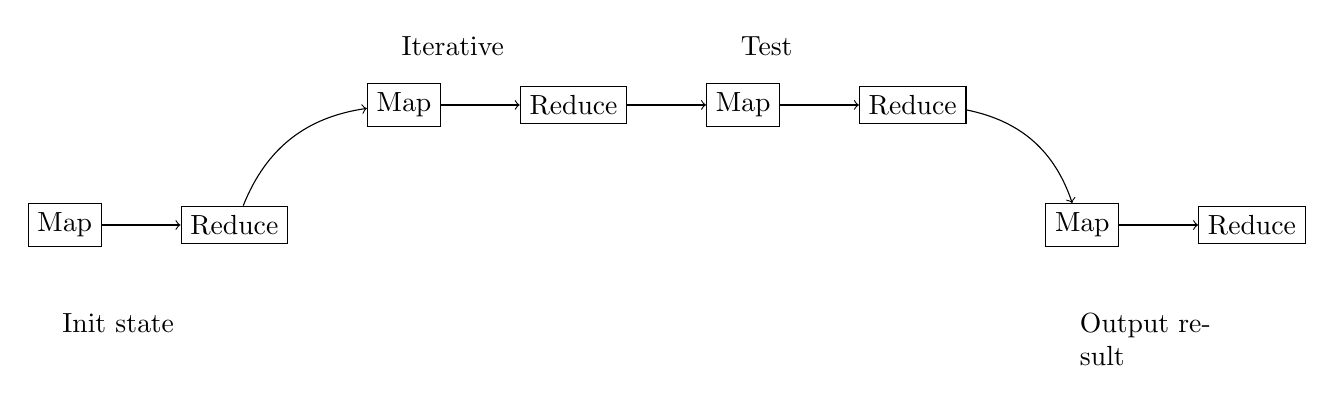
\begin{tikzpicture}
    \node[rectangle, draw] (IM) {Map};
    \node[rectangle, draw, right= of IM] (IR) {Reduce};

    \node[rectangle, draw, above right= of IR] (CM) {Map};
    \node[rectangle, draw, right= of CM] (MR) {Reduce};

    \node[rectangle, draw, right= of MR] (TM) {Map};
    \node[rectangle, draw, right= of TM] (TR) {Reduce};

    \node[rectangle, draw, below right= of TR] (OM) {Map};
    \node[rectangle, draw, right= of OM] (OR) {Reduce};

    \draw (IM) edge[->] node[below=1cm, text width=2cm] {Init state} (IR);
    \draw (CM) edge[->] node[above=0.5cm, text width=2cm] {Iterative} (MR);
    \draw (TM) edge[->] node[above=0.5cm, text width=2cm] {Test} (TR);
    \draw (OM) edge[->] node[below=1cm, text width=2cm] {Output result} (OR);

    \draw (IR) edge[->, bend left] (CM);
    \draw (MR) edge[->, ] (TM);
    \draw (TR) edge[->, bend left] (OM);
\end{tikzpicture}

Iterative MapReduce can be done if the reduce
output is compatible with map input but this require to passing the
entire state and doing a lot of network and disk I/O.


\subsection{Graphs algorithm}
$G = (V, E)$ where $V$ is vertices, $E$ edges of the form $(v_1, v_2, cost, attr)$
where $v_1, v_2 \in V$.

\begin{itemize}
    \item \textbf{Single Source Shortst Path (SSSP)}: based on dijkstra algorithm idea but parallelized.
        \begin{description}
            \item[Init]: for each node $id$, $<\infty, -, \{<succId, cost>\}>$
            \item[Map]: for each node $id$, $<dst, next, \{<succId, cost>\}>$:
                \begin{itemize}
                    \item emit $id$, $<dst, next, \{<succId, cost>\}>$
                    \item for each successor:
                        \begin{itemize}
                            \item emit $succId, <dst+cost, id>$ 
                        \end{itemize}
                \end{itemize}
            \item[Reduce]: emit $id$, $<minDst, nextWithMinDst, \{<succId, cost>\}>$
        \end{description}

        This algorithm is based on a \textit{wave} which go on at each iteration.

    \item \textbf{k-clustering}: the idea is to assign $k$ random centroid and move them 
        until be stable.
        \begin{description}
            \item[Init]: choose random point
            \item[Map]: Assign each point to the closest centroid
                $$S_i^{(t)} = \{ x_j : x_j − m_i^{(t)} ≤ x_j − m_i^{(* t )} , i* = 1,..., k \}$$
            \item[Reduce]: Recenter with $m_i$ the new centroid for its points
                $$m_i^{(t+1)} = \frac{1}{|S_i^{(t)}|} \sum_{x_j \in S_i^{(t)}} x_j$$
        \end{description}

    \item \textbf{Classification with naïve Bayes}: where it's \textit{naïve} because probability
        of events are independent.
        $$\textrm{Probability messages "XYZ" is SPAM?} = \frac{p(spam) p(containsXYZ | spam)}
        {p(containsXYZ)}$$ 

        \begin{itemize}
            \item \texttt{p(spam)} : Nbr spam email / Nbr email
            \item \texttt{p(containsXYZ)} : Nbr emails with XYZ / Nbr emails
            \item \texttt{p(containsXYZ|spam)} : Nbr emails with XYZ / Nbr emails with XYZ
        \end{itemize}

        \begin{tabular}{m{2cm}cm{13cm}}
            Nbr spam with XYZ &:
            & 
            \begin{description}
                \item[map]: for each message $m <class, \{words\}>$, emit $<word, class> \rightarrow 1$
                \item[reduce]: emit $<word, class> \rightarrow count$
            \end{description}
        \end{tabular}

        \begin{tabular}{m{2cm}cm{12cm}}
            Nbr email with XYZ&:
            & 
            \begin{description}
                \item[map]: for each message $m <class, \{words\}>$, emit $<word> \rightarrow 1$
                \item[reduce]: emit $<word> \rightarrow count$
            \end{description}
        \end{tabular}

    \item \textbf{PageRank}: The idea is to allow $\frac{1}{N}$ vote par page
        at the initialization, and each page vote for all the page it has a
        link to. To ensure fairness, pages voting for more than one page must
        split their vote equally between them. Voting proceeds in rounds: in
        each round, each page has the number of votes it received in the
        previous round.


        \begin{itemize}
            \item \textsc{Random surfer model}: Imagine a random surfer, who starts on a 
                random page and, in each step
                \begin{enumerate}
                    \item Click on a random link on the page with probability $d$ 
                    \item Jump to a random page with probability $1-d$ 
                \end{enumerate}
                The PageRank of a page can be interpreted 
                as the fraction of steps the surfer spends on 
                the corresponding page


            \item \textsc{Naïve PageRank}
                $$rank_i = \sum_{j \in B_i} \frac{1}{N_j} rank_j \quad \textrm{where }N_i \textrm{ is
                the outgoing link of i and} B_i \textrm{ the ingoing link of i}$$ 

                This can't be able to manage vertex which have no outgoing edge.

                \begin{tabular}{m{7cm}m{7cm}}
                    \textbf{Sinks} & \textbf{Hogs}\\
                    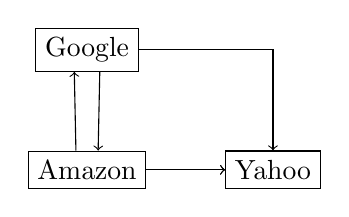
\begin{tikzpicture}
                        \node[rectangle, draw] (G) {Google};
                        \node[rectangle, draw, below= of G] (A) {Amazon};
                        \node[rectangle, draw, right= of A] (Y) {Yahoo};

                        \draw[->] (G) -| (Y);
                        \draw[->] (G.300) -- (A.60);
                        \draw[<-] (G.240) -- (A.120);
                        \draw[->] (A) -- (Y.180);
                        \draw[->] (A) -- (Y.180);
                    \end{tikzpicture}
                    &
                    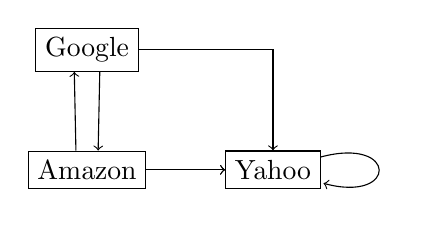
\begin{tikzpicture}
                        \node[rectangle, draw] (G) {Google};
                        \node[rectangle, draw, below= of G] (A) {Amazon};
                        \node[rectangle, draw, right= of A] (Y) {Yahoo};

                        \draw[->] (G) -| (Y);
                        \draw[->] (G.300) -- (A.60);
                        \draw[<-] (G.240) -- (A.120);
                        \draw[->] (A) -- (Y.180);
                        \draw[->] (A) -- (Y.180);
                        \draw[->, loop right] (Y) edge[loop right] (Y);
                    \end{tikzpicture}\\
                    PageRank is lost after each round and $\forall_i rank_i = 0$ & 
                    PageRank is accumulates on Yahoo and $\forall_i rank_i = 0$ behalf 
                    $rank_{yahoo} = 1$
                \end{tabular}

            \item \textsc{Improved PageRank}
                $$rank_i = 1-d + d \sum_{j \in B_i} \frac{1}{N_j} rank_j \quad \textrm{where }N_i \textrm{ is
                the outgoing link of i and} B_i \textrm{ the ingoing link of i}$$ 
        \end{itemize}

        \begin{description}
            \item[Init]: page $p <1/Nn, \{outgoingLink\}>$
            \item[Map]: page $p$ propagate $\frac{1}{N_p} * d * weigth_p$
            \item[Reduce]: page $p$ = $1-d + \sum_{incomingWeight}$
        \end{description}

\end{itemize}


\section{Hadoop}

\subsection{HDFS}
Hadoop use a distributed file system (HDFS) specialized for particular
types of applications. Files are stored as sets of blocks (64MB) which
are replicated for durability and availability.

\begin{center}
    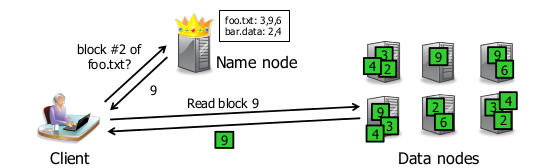
\includegraphics[width=11cm]{img/hdfs}
\end{center}

\begin{itemize}
    \item Namespace is managed by a single name node and transfert
        is done directly between client and data node
    \item State stored in two files:

        \begin{tabular}{m{7cm}m{9cm}}
            \begin{itemize}
                \item fsimages: snapshot of file system metadata
                \item edits: change since last snapshot
            \end{itemize} 
            &
            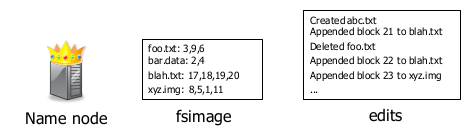
\includegraphics[width=9cm]{img/namenode}
        \end{tabular}
\end{itemize}
If the state of the namenode is lost, there are two possible solutions:
\begin{itemize}
	\item \textbf{Metadata backups} Namenode can write its metadata to a local disk
	and/or to a remote NFS
	\item \textbf{Secondary Namenode} (1) Periodically merge the edit log with fsimage 
	to prevent from growing to large, (2) Copy of the metadata
\end{itemize}
\paragraph{Note} Secondary namenode is more of a checkpoint
\footnote{http://blog.madhukaraphatak.com/secondary-namenode---what-it-really-do/} 
than a backup node, if it fails
$\to$ data loss.



\begin{table}[!h]
    \begin{tabular}{m{8cm}m{8cm}}
        \textbf{Does well} & \textbf{Does not well} \\
        \begin{itemize}
            \item very large read-only or append-only file (Terabytes EASY)
            \item Sequential access parten
            \item High throughput and high capacity
        \end{itemize} 
        &
        \begin{itemize}
            \item Low-latency access
            \item Multiple writers
            \item Not append-only file
            \item Storing small files
        \end{itemize} \\
        & $\rightarrow $ This is well done by Network File System (NFS)
    \end{tabular}
    \caption{HDFS advantage}
\end{table}


\subsection{Hive Query Language (HQL)}
A data warehouse infrastructure built on top 
of Hadoop for providing data summarization, 
query and analysis.

\subsubsection{SQL recap}
\begin{itemize}
    \item \texttt{SELECT}: Projection and remapping/renaming 
    \item \texttt{JOIN}: Cartesian product 
    \item \texttt{WHERE}: Filtering 
    \item \texttt{UNON, INTERSECT}: Set operations 
    \item \texttt{GROUP BY, MIN, MAX, AVG}: Aggregation 
    \item \texttt{ORDER BY}: Sorting 
    \item \texttt{SELECT .. FROM (SELECT .. FROM ..)}: Composition 
\end{itemize}

\subsubsection{HQL}

\begin{itemize}
    \item Suitable for processing structured data
    \item Create a table structure on top of HDFS
    \item Queries are compiled in to MapReduce jobs
\end{itemize}
\paragraph{Note} Hive is not designed fot OnLine Transaction Processing which 
consist mostly of updates. Indeed updating record or transaction are not 
supported

\subsection{Pig and Pig latin}
Relational data model does no allow nested table (attribute which is collection).
That's a part of what Pig Latin brings.

Somewhere between a programming language and a DBMSa which allows
distributed  programming with explicit parallel dataflow operators.

\begin{description}
    \item[Pig]: runtime system
    \item[Pig latin]:
        A dataflow language that compiles to MapReduce.
        Collection-­valued   expressions  whose  results  get  
        assigned  to  variables.
        \begin{itemize}
            \item A  program  does  a  series  of  assignments  in  a  dataflow
            \item It  gets  compiled  down  to  a  sequence  of  MapReduces. 

                Note that Pig Latin has its own query langage (not SQL)
        \end{itemize}
\end{description}

\subsubsection{Basic SQL-like operation}
Operations are \textbf{explicitly} specified.
\begin{itemize}
    \item \texttt{load\ldots as}: Projection and renaming 
    \item \texttt{foreach \ldots generate}: remapping 
    \item \texttt{filter by}: Filtering 
    \item \texttt{join}: intersection 
    \item \texttt{group by}: Aggregation 
    \item \texttt{order}: Sorting 
    \item \texttt{store}: save result
\end{itemize}

\subsubsection{Implementation}
\begin{center}
    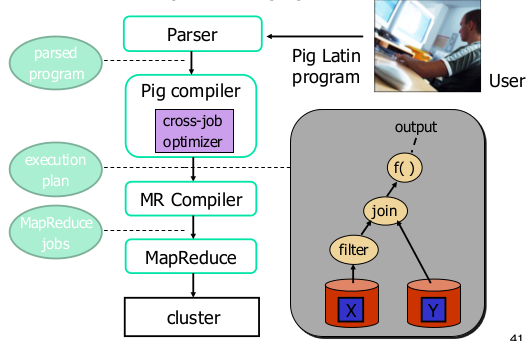
\includegraphics[width=10cm]{img/pig}
\end{center}

\subsubsection{Work-sharing techniques}

\begin{center}
    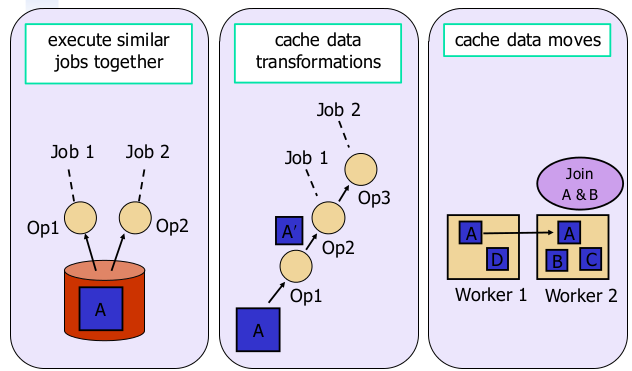
\includegraphics[width=10cm]{img/work}
\end{center}


\section{Batch processing}
\subsection{Pregel: Bulk Synchonous Parallel}
Much  of  the  mismatch  stems  from  the  lack  of  shared  global  state.
Complex  applications  and  interactive  queries  both  need  one  thing  that
MapReduce lacks: efficient  primitives  for  data  sharing.


With \textbf{Pregel}, we consider the  nodes  with a  state  (memory)  
that  carries  from  superstep to  superstep.

\subsubsection{Model}

It's a sequence of \textbf{superstep} where at superstep $S$:
\begin{enumerate}
    \item Compute in parallel at each $V$
        \begin{itemize}
            \item Read message sent to $V$ in $S-1$
            \item Update value/state
            \item Optionnaly change topology
        \end{itemize}
    \item Send messages to neighbors
    \item Synchronization
\end{enumerate}

\begin{tabular}{m{9cm}m{7cm}}
    $\rightarrow $ Algorithm terminates when all vertices are simultaneously inactive.
    & 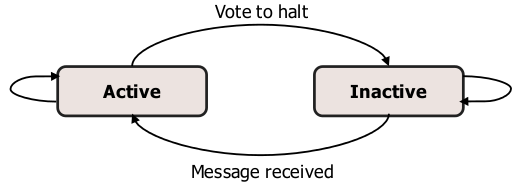
\includegraphics[width=7cm]{img/halt}
\end{tabular}

\subsubsection{Algorithm}
\begin{itemize}
    \item \textbf{Find Maximum Value}

        \begin{tabular}{m{11cm}m{5cm}}
            \begin{enumerate}
                \item At superstep 0, propagating value to neighbors
                \item In each step, if he learn a larger number, then propagate
                    it to neighbors else vote to halt
                \item Finish when all vote halt
            \end{enumerate}
            & 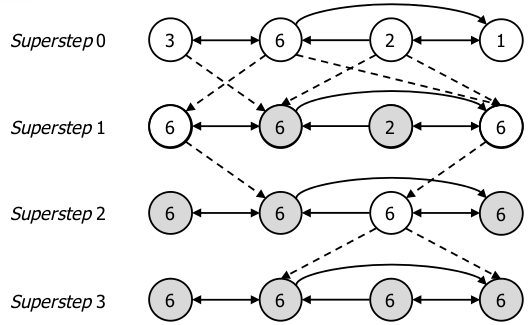
\includegraphics[width=5cm]{img/FMV}
        \end{tabular}

    \item \textbf{PageRank}
        $$rank_i = 1-d + d \sum_{j \in B_i} \frac{1}{N_j} rank_j \quad \textrm{where }N_i \textrm{ is
        the outgoing link of i and} B_i \textrm{ the ingoing link of i}$$ 

        \begin{itemize}
            \item Each  page  $j$  distributes  its  importance  to  all  of  the  pages  it  
                points  to  (so  we  scale  by  $\frac{1}{N_j}$)
            \item Page  p’s  importance  is  increased  by  the  importance  of  its  
                back  set
        \end{itemize}
        %TODO: example pregel code ?

\end{itemize}


\subsection{Spark: Resilient Distributed Dataset}

Basically, Spark is a distributed  memory  abstraction  that  is  both  fault-­tolerant  
and  efficient. Note that there is some restriction form of distributed shared memory
in order to be called \textit{Resilient Distributed Datasets (RDDs)}
\begin{itemize}
    \item Immutable, partitioned collections of records
    \item Can  only  be  built  through  coarse-­grained deterministic  
        transformations  (map,  filter,  join,  ...)
\end{itemize}

Despite their restrictions,  RDDs can express many parallel algorithms (These
naturally  apply the same operation to many items). RDDs also unify many
programming models.

\begin{tabular}{m{7cm}cm{7cm}}
    \begin{itemize}
        \item MapReduce,  DryadLINQ
        \item Pregel graph  processing
        \item Iterative  MapReduce
        \item SQL:  Hive  on  Spark  (Shark)
    \end{itemize}
    & $\Rightarrow$  &
    All are based on coarse-­grained  
    operations
\end{tabular}

\begin{center}
    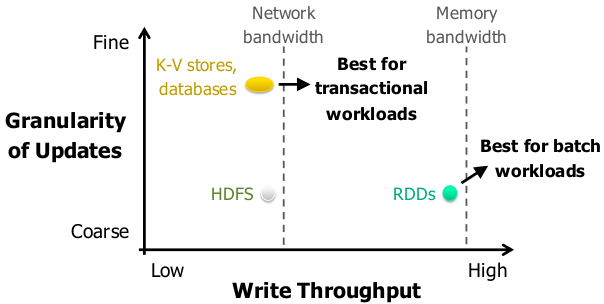
\includegraphics[width=11cm]{img/databaseComp}
\end{center}

\subsubsection{Efficient fault recovery}
Spark use \textbf{lineage}:

\begin{tabular}{m{9cm}m{7cm}}
    \begin{itemize}
        \item Log  one  operation  to  apply  to  many  elements
        \item Recompute lost  partitions  on  failure
        \item No  cost  if  nothing  fails
    \end{itemize}
    &
    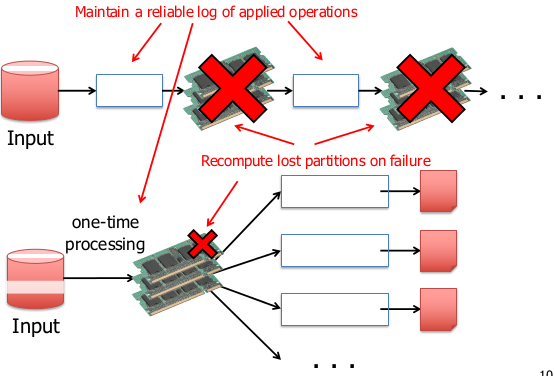
\includegraphics[width=7cm]{img/sparkFault}
\end{tabular}

\subsubsection{Spark operation}
\begin{itemize}
    \item Transformations (define a new RDD) : \begin{tabular}{ccc}
            map & flatMap & union \\ join & cogroup & cross \\ mapValues & filter & sample\\
            groupByKey & reduceByKey& sortByKey\\
        \end{tabular}

    \item Action (return a result to driver program) : \begin{tabular}{ccc}
            collect& reduce& count\\ save& lookupKey& take\\
        \end{tabular}
\end{itemize}

\subsubsection{Spark scheduler}

\begin{tabular}{m{7cm}m{8cm}}
    \begin{itemize}
        \item Pipelines  functions within  a  stage
        \item Locality  \&  data  reuse aware
        \item Partitioning-­aware to  avoid  shuffles
    \end{itemize}
    &
    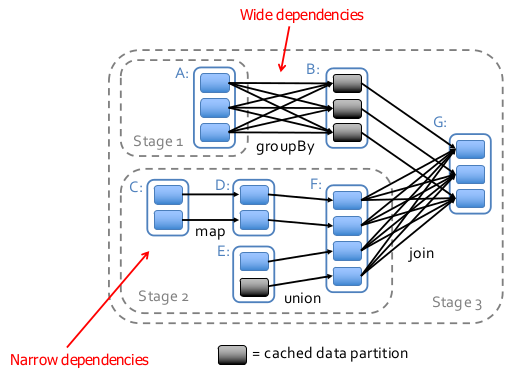
\includegraphics[width=8cm]{img/sparkScheduler}
\end{tabular}

\subsubsection{Algorithm}
\begin{itemize}
    \item \textbf{PageRank}:
        $$rank_i = 1-d + d \sum_{j \in B_i} \frac{1}{N_j} rank_j \quad \textrm{where }N_i \textrm{ is
        the outgoing link of i and} B_i \textrm{ the ingoing link of i}$$ 

        \begin{lstlisting}[mathescape]
        var links   =  //  RDD  of  (url,   neighbors)   pairs
        var ranks   =  //  RDD  of  (url,   rank)   pairs
        for  (i $\leftarrow$ 1 to ITERATIONS)   {
            contribs =  links.join(ranks).flatMap {
                (url,   (links,   rank))   =>
                links.map(dest =>  (dest,   rank/links.size))
            }
            ranks   =  contribs.reduceByKey((x,   y)  =>  x  +  y)
            .mapValues(sum   =>  0.85*sum   +  0.15/N)
        }
        \end{lstlisting}
        Note that as RDDs are  immutable, contribs and  ranks  are  new  RDDs!

        %TODO optimizing placement slide 20 for 07
\end{itemize}


\section{Stream processing}
Many important applications must process large streams of live data
and provide results in near-­real-­time.
Distributed  stream  processing  framework  is  required  to  scale  large
clusters  (100s  of  machines) and achieve  low  latency  (few  seconds).


\begin{tabular}{m{10cm}m{6cm}}
    Streaming  systems  have  a  record-at-a-time processing  model
    \begin{itemize}
        \item Each node has mutable state
        \item For  each  record,  update  state   and  
            send  new  records
    \end{itemize}
    &
    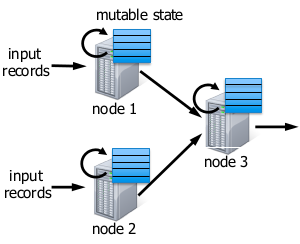
\includegraphics[width=5cm]{img/stream}
\end{tabular}

Note that state  is  lost  if  node  dies, so make a stateful stream
processing  be  fault-­tolerant  is  challenging.

\subsection{Storm}

Framework  for  distributed  stream  processing which provides:  
(1) stream  Partitioning, (2) fault  tolerance  and (3)  parallel  execution.
\begin{center}
    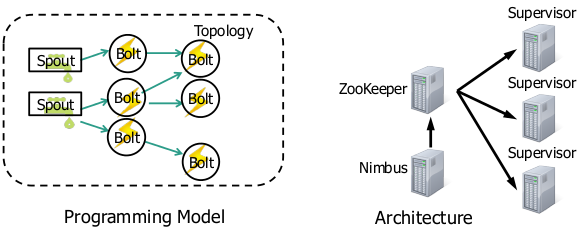
\includegraphics[width=10cm]{img/storm}
\end{center}

\begin{itemize}
    \item \textbf{Spout} is the source of stream where \textbf{bolt} process the stream
        and output new streams
    \item Nimbus  node  (master  node): 
        \begin{enumerate}
            \item Distributes  code,  launches  workers  across  the  cluster
            \item Monitors  computation  and  reallocates  workers  as  needed
        \end{enumerate}
    \item ZooKeeper nodes (coordinate  the  cluster)
    \item Supervisor  nodes: Start  and  stop  workers  according  to  signals
        from  Nimbus
\end{itemize}

\subsubsection{Fault tolerance}
Storm  can  guarantee  that  every  tuple  will  be  process  at  least  once or
at  most  once,  but  not  exactly  once. (Exactly  once  guarantee  requires
a  durable  data  source  that  can  replay  any  message  or  set  of
messages  given  the  necessary  selection  criteria)
%Suppose you want to update a counter in a database, if a worker fails, you 
% don't know if it has failed before updating the value or after 
%TODO really see slide 29 for 07 why this


If  a  supervisor  node  fails,  Nimbus  reassigns  that  node’s  task  to
other  nodes  in  the  cluster. Any  tuples  sent  to  a  failed  node  will
time  out  and  be  replayed. (Delivery  guarantee  dependent  on  a  reliable
data  source)

\subsection{Spark streaming}
Run  a  streaming  computation  as  a  series  of  
very  small,  deterministic  batch  jobs. This 
combine  the  efficiency  of  in-­memory  
distributed   processing  of  Spark  with  stream  
processing  mode.


\subsubsection{Work}

\begin{tabular}{m{10cm}m{6cm}}
    \begin{itemize}
        \item Chop  up  the  live  stream  into  batches  of  X  seconds  
        \item Spark  treats  each  batch  of  data  as  RDDs  and  processes  them
            using  RDD  operations
        \item Finally,  the  processed  results  of  the  RDD  operations  are
            returned  in  batches
    \end{itemize}
    &
    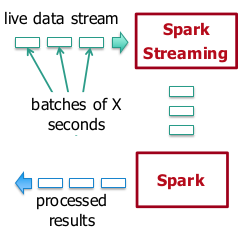
\includegraphics[width=4cm]{img/sparkStream}
\end{tabular}

At the end, a new RDDs are created for every batch

\subsubsection{Fault tolerance}

\begin{tabular}{m{10cm}m{6cm}}
    \begin{itemize}
        \item RDDs  remember  the  operations  that  created  them.
        \item Batches  of  input  data  are  replicated  in  memory  for
            fault-­tolerance.
        \item Data  lost  due  to  worker  failure,  can  be  recomputed  from
            replicated  input  data.
    \end{itemize}
    &
    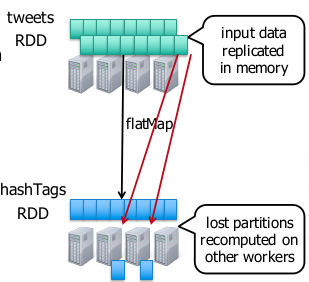
\includegraphics[width=6cm]{img/faultSpark}
\end{tabular}


\section{Data Center Galaxy}

\subsection{Infrastructure}

\begin{tabular}{m{8cm}m{7cm}}
    Streaming  systems  have  a  record-at-a-time processing  model
    \begin{itemize}
        \item Servers organized in racks with a Top Of Rack (ToR) switch
        \item Aggregation switch interconnect ToR switch
    \end{itemize}
    &
    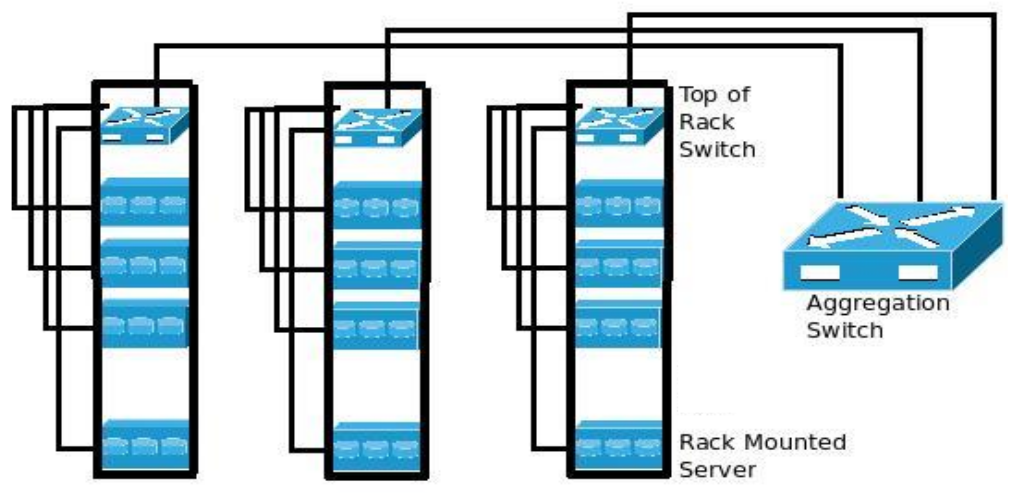
\includegraphics[width=7cm]{img/dcStruct}
\end{tabular}

\subsection{Traffic}

\paragraph{Internal traffic}

Internal traffic (East-west) is clearly a critical component compared
to external traffic (North-south).
\begin{center}
    \begin{tabular}{m{7cm}m{7cm}}

        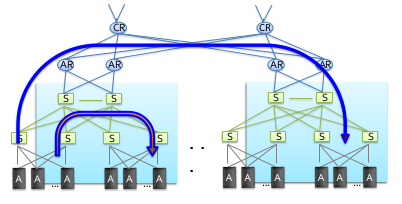
\includegraphics[width=7cm]{img/internalCrit}
        &
        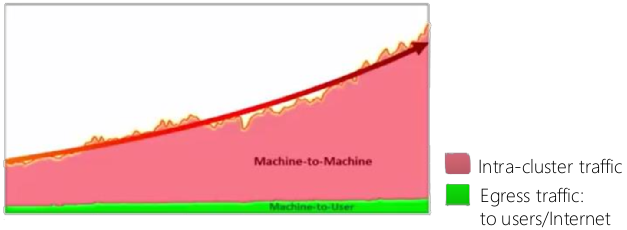
\includegraphics[width=7cm]{img/internalTraffic}
    \end{tabular}
\end{center}

\subsubsection{Solutions}

\begin{tabular}{m{12cm}m{4cm}}
    The goal is to allow each server to talk to any other server at its full access
    link rate.
    We can see the DC as a giant switch between server.
    &
    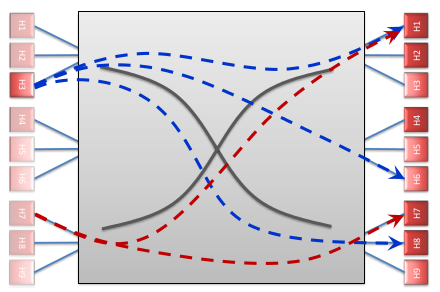
\includegraphics[width=3cm]{img/giant}
\end{tabular}

\begin{itemize}
    \item \textbf{Full Bisection Bandwith }: it's the \textit{scale up } approach.

        \begin{tabular}{m{11cm}m{7cm}}
            A traditional tree topology is really expensive
            because it requires a lot of switch with high bandwidth.
            &
            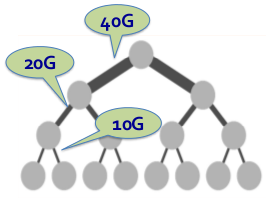
\includegraphics[width=3cm]{img/FBBW}
        \end{tabular}

        \paragraph{Oversubscription}
        A solution is to provision less
        than full Bisection Bandwidth because we can reasonably say
        that all server will know talk with all server simultaneously. 


    \item \textbf{Fat Tree}: it's the \textit{scale out} approach.

        \begin{tabular}{m{11cm}m{7cm}}
            Fat tree offers high bisection bandwidth but
            the system must be to exploit this available capacity:
            \begin{itemize}
                \item Routing must use all path
                \item Transport protocol must fill into all pipe
            \end{itemize}

            Note that this topology only require 10Gb/s links.
            &
            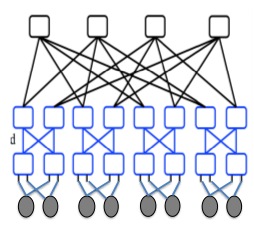
\includegraphics[width=3cm]{img/fattree}
        \end{tabular}
\end{itemize}

\subsection{Network stack}


\paragraph{Models}
Traditional \textbf{TCP} enforce \textit{per-flow min/max fairness}, but
Data center operators want to enforce other models such
as tenant-based or deadline-based.

\paragraph{Low latency}
\begin{itemize}
    \item 55\% of flow $<100KB$ $\Rightarrow$ Delay-sensitive
        So low latency is \textbf{critical}!
    \item 5\% of flow $>10MB$ $\Rightarrow$ Throughput-sensitive
\end{itemize}

\begin{center}
    \begin{tabular}{cc}
        High throughput & Low latency\\
        \hline
        Deep queue at switches& Shallow queues at switches \\
        which increase delays & which
        is bad for burst and throughput\\
    \end{tabular}
\end{center}

The goal is to have in DC low queue occupancy (to achieve
low RRTs within DC approache $1µs$) and high throughput.


\subsubsection{Solutions}
\begin{itemize}
    \item \textbf{DC-TCP} which use \textbf{Explicit Congestion Notification (ECN)} 
        \begin{enumerate}
            \item React early and quickly by using ECN which avoid large
                buildup in queue and allow low latency!

                \paragraph{Switch} If queue length > $k$ set ECN bit

            \item React in proportion to the extend of congestion, not
                in presence.

                \paragraph{Sender} Maintain running average of \textbf{fraction
                of packets marked} ($\alpha$)
                $$ alpha = (1-g) \alpha + g \frac{\# marked ACK}{\# ACK} $$
                and adapts the window based on $\alpha$
                $$ W = (1-\frac{\alpha}{2}) W$$
        \end{enumerate}

    \item \textbf{pFabric}: use priorities
        \begin{enumerate}
            \item Packets carry a single priority number.

                priority = remaining flow size (e.g., \#bytes un-acked)

            \item Switches have small queues (10 packets), send highest
                priority and drop lowest priority

            \item Server (re)transmit aggressively it means at full link rate
                and drop transmission rate only under extreme loss (timeout).
        \end{enumerate}
\end{itemize}

\paragraph{Flow Completion time (FCT)}: is
the time from when flow started at the sender, to when all
packets in the flow were received at the receiver.
\paragraph{Pfabric} With DCTCP, small flow are delayed by big ones. To
handel that:
\begin{itemize}
	\item Packets carry a single priority number representing the remaining flow size.
	\item Switches send the packet with highest priority and drop the lowest
	priority packet
	\item Servers transmit/retransmit at full link rate and decrease transmission
	rate only under extreme loss (typically timeouts)
\end{itemize}
assigning priority number to packet. 
\begin{center}
    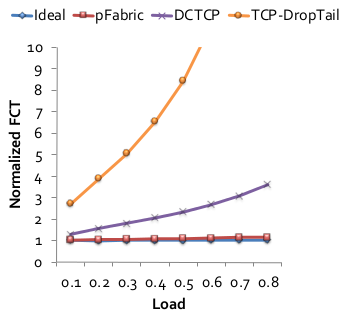
\includegraphics[width=8cm]{img/fct}
\end{center}

\subsection{Management}

\begin{description}
    \item[Data plane]: 
        \begin{tabular}{m{8cm}m{3cm}}
            process packet by using local forwarding state and packet header.
            &
            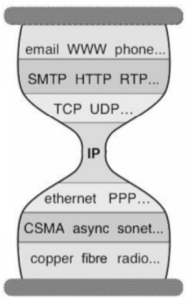
\includegraphics[width=2cm]{img/app}
        \end{tabular}
    \item[Control plane]: Compute forwarding state.

        Actually, we have a protocol which solve
        \begin{itemize}
            \item Consistent with particular low-level hardware/software
            \item  Based on entire network topology
            \item  For all routers/switches (i.e., must configure each one)
        \end{itemize}

        But it's too much, and \textbf{SDN} allow to perform some abstraction.
\end{description}

\subsubsection{Software Defined Network (SDN)}
\begin{center}
    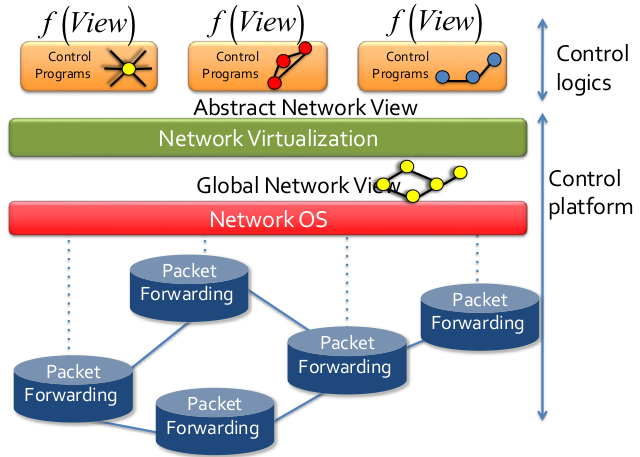
\includegraphics[width=8cm]{img/SDN}
\end{center}

\subsubsection{Open Flow}
is a protocol for remotely controlling the forwarding table of a switch or
router which is one element of SDN.

\begin{tabular}{m{8cm}m{8cm}}
    \begin{itemize}
        \item Message between controller and switches 
            (Synchronous: Stats, Flow-mods, Asynchronous: Packet-in)
        \item Abstract hardware details
        \item  Allows direct control over forwarding table
    \end{itemize}
    &
    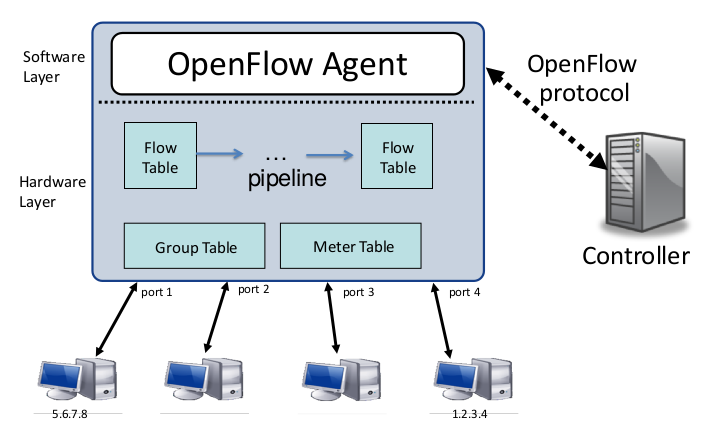
\includegraphics[width=9cm]{img/openflow}
\end{tabular}

\begin{table}[ht!]
	\centering
	\begin{tabular}{|c|l|}
	\hline
	Match field & To match against packet. These consist of the ingress port 
	and packet headers\\
	\hline
	Priority & Matching precedence of the flow entry\\
	\hline
	Counters & e.g. packet and byte counters\\
	\hline
	Instructions & Determine action set or pipeline processing\\
	\hline
	Timeouts & Maximum amount of time or idle time before flow is expired by
	the switch\\
	\hline
	Cookies & Opaque data value chosen by the controller. Not used when
	processing packets.\\
	\hline
	\end{tabular}
	\caption{Flow table entries}
\end{table}

\begin{table}[ht!]
\begin{tabular}{|c|c|c|c|c|c|c|c|c|c|c|c|}
	\hline
	Switch&VLAN&VLAN&MAC&MAC&Eth&IP&IP&IP&IP&L4&L4\\
	Port&ID&pcp&src&dst&type&src&dst&Tos&Prot&sport&dport\\
	\hline
\end{tabular}
\caption{match fields}
\end{table}
\begin{table}[ht!]
	\centering
	\begin{tabular}{|c|c|l|}
	\hline
	Message&Direction&Description\\
	\hline
	Packet-In & Switch$\to$Controller & Transfer the control of the packet to the 
	controller.\\
	&& Packet-in events can be configured to buffer packets.\\
	\hline
	Packet-Out & Controller $\to$ Switch & Instruct switch to send a packet out 
	of a specified port.\\
	&& Send in response to Packet-in messages.\\
	\hline
	Modify-State & Controller$\to$ Switch & Add,delete and modify flow/group entries
	in the flow tables\\
	&& and to set switch port properties.\\
	\hline
	Flow-Removed & Switch $\to$ Controller & Inform the controller about the removal
	of a flow entry \\
	&&from a flow table.\\
	\hline
	\end{tabular}
	\caption{messages exchanged in openFlow}
\end{table}

%TODO improvement from 89 for 08


\section{Web programming}

\begin{itemize}
    \item \textbf{HTML}: Separate content and style by using CSS.
    \item \textbf{Browser}: Show information and not the part of the file 
        which say how to show information.

    \item \textbf{Delivering document} 
        \begin{enumerate}
            \item Peer to peer model
            \item Client/server model where a 
                server is a machine that offer services to other machine.

                Note that state must be maintain when request are related. 
                \begin{itemize}
                    \item Client side: It's better to keep state on client side to avoid DoS.
                    \item Server: If state is on the server and multiple server are used,
                    they must be able to exchange state information.
                \end{itemize}

                \paragraph{Concurrency}
                \begin{itemize}
                    \item Thread pools: keep a thread pool with a fixed number of 
                        worker threads
                    \item Event-driven: server's work is driven by events
                        which need a single thread.
                \end{itemize}

                Event-driven servers typically have better performance
                and do not need as much synchronization but
                thread-based are easier to write and maintain.

                \paragraph{Multiple machine}
                Need a proxy to load balance request across machines.

        \end{enumerate}

    \item \textbf{Uniform  Resource  Identifier (URI)} which comme in two form:
        \begin{enumerate}
            \item Uniform  Resource  Name (URNs): \textit{What} to find
            \item Uniform  Resource  Locator (URLs): \textit{Where} to find
        \end{enumerate}

    \item \textbf{DNS}: Hierarchical namespace

        \begin{tabular}{m{5cm}m{11cm}}
            Authoritative  server  knows,  for  each  name  in  its  zone,  which
            machine  corresponds  to  a  given  name,  or  which  other  name  server
            is  responsible.
            &
            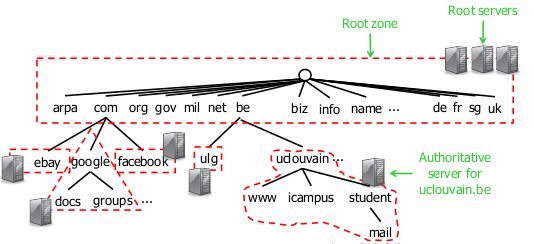
\includegraphics[width=11cm]{img/dns}
        \end{tabular}

    \item \textbf{HTTP}: is a simple stateless protocol
        which use request/response that contain headers used to
        exchange additional information.

        \begin{enumerate}
            \item GET: retreive document
            \item HEAD: Get metadata for a specific document
            \item POST: Add information to a document (as form)
            \item PUT, DELETE
        \end{enumerate}

    \item \textbf{Dynamic content}:

        \paragraph{Document Object Model} (DOM)
        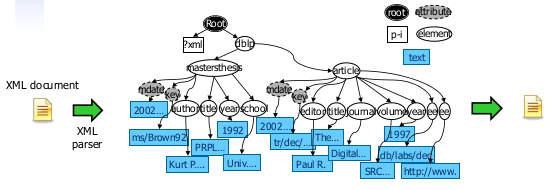
\includegraphics[width=11cm]{img/dom}

        \paragraph{XMLHttpRequest}
        It's a JavaScript  object  that  enables  web  pages  
        to  dynamically and asynchronously  load  more  content. 

        \paragraph{Event handlers}
        Events  can  be  requested  from  the  web  page
        or  directly  from  JavaScript.

        \begin{itemize}
            \item Server-side
                \begin{itemize}
                    \item Web app
                        \begin{enumerate}
                            \item Common Gateway Interface (CGI). When
                                dynamic content is requested:
                                (1) the web server prepare metadata and user-submitted
                                data, (2) runs an external program that produce the web page and
                                (3) return the web page produce by program to the client
                            \item Java servlets: servlets implement a specific
                                method that is given request. They also run one
                                \textbf{servlet container} and each request is its own
                                thread.
                        \end{enumerate}

                        \begin{center}
                            \begin{tabular}{l|cc}
                                & CGI & Servlets \\
                                \hline
                                Request handled by & Processes & Threads \\
                                Copies of code & Potentially many & One \\
                                Session state stored & File System & Servelt container \\
                                Security & Problematic & Handled by Java sandbox \\
                                Portability & Varies & Java \\
                            \end{tabular}
                        \end{center}

                    \item Node.js which is a event-driven programming model, so there
                        is a single thread which must never block. 

                        Note that Express are minimal and flexible framework for writing
                        web app in node.js and EJS allow to write \textit{page templates}.

                \end{itemize}


            \item Client-side
                \begin{itemize}
                    \item JavaScript: Can be embed entirely in HTML or attach in
                        a separate file.

                    \item Ajax: Asynchronous JS, XML,...
                        \begin{description}
                            \item[+] Much more responsive than plain HTML
                            \item[-] Difficult to integrate navigation element (back button),
                                to accommodate search engine, some compatibility issues
                        \end{description}
                        \begin{center}
                            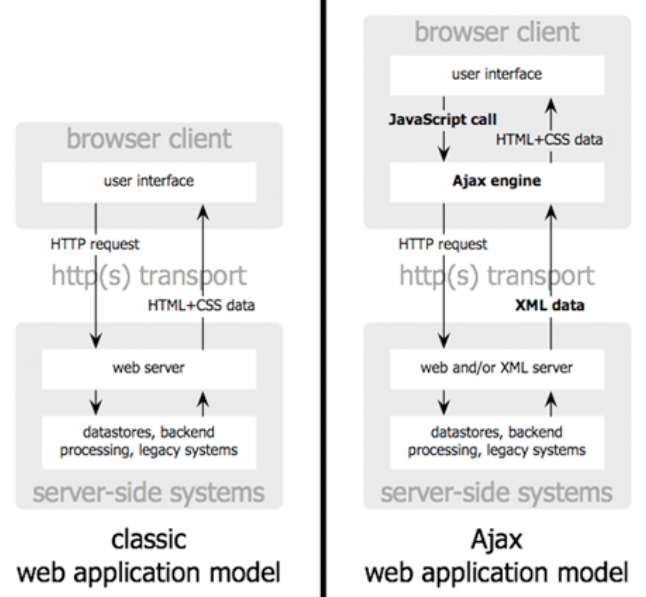
\includegraphics[width=9cm]{img/ajax}
                        \end{center}
                \end{itemize}
        \end{itemize}

    \item \textbf{Session management}
        \begin{itemize}
            \item Use session ID in part of every URL:
                \begin{enumerate}
                    \item URL rewriting by append session ID
                        $$<a  href="foo.html">  \rightarrow <a  href="foo.html?sid=012345">$$
                    \item hidden session ID variables in the HTML
                        $$<input  type="hidden"  name="sid"  value="012345">$$
                \end{enumerate}

            \item Use cookies which is a set of key-­value pairs that a web
                site can store in your browser which is send with \texttt{set-cookie header}
                in HTTP response.

                \paragraph{Note}
                Each cookies as an expiration date, a domain and a
                path. Browser  only  sends  the  cookies  whose  path  
                and  domain  match  the  requested  page.

                \paragraph{Issue}
                Cookie persist and can have some useful information such as
                password.
        \end{itemize}
\end{itemize}

\section{Behavioural tracking}

The idea is to make the client load a blank pixel so that it reportes its activity to the server. Motivations are :
\begin{description}
\item[Operational] logging, payment reports
\item[Product] create analytics, recommendation
\item[Insight] analytics, research
\end{description}

\subsection{Production}
Client side implementation. Javascripts that will schedule and plan for HTTP Calls. Will have to handle failure. Send status of the client to the server. The platform matters as mobile can have battery drain issue. So, need for keep alive, scheduling, batching. All of these can be achieve via the device ID and the local storage of the browser.

\subsection{Collection}
The collection is the front door of the pipeline. It is servers that needs high availability (HA). This can be done via round-robin DNS and HA proxy that will redirect the HTTP flow to collectors.

\subsection{Transmission}
All the collectors need to send the collected data to a big queue that will process them. For this task, we need guarantee on delivery, high availibility and queuing behavior.

For the guarantee on delivery, this problem is complex. In an ideal case, you send the message, get an acknowledgment. But as the queue service is distributed, it gets more complicated. If the ack is lost, you're going to send the message a second time. So you will have a de-duplication. But it ensures that you have ``at least once'' the message. To tackle this problem and get ``exactly Once'' the message, you can put a filter behind the queue. But this will cost in performance.

Two solutions proposed by the paper : kafka and RabbitMQ.
\begin{tabular}{l|r}
RabbitMQ & Kafka \\
\hline
\hline
Master/slave & Masterless\\ 
Complex topology & Zookeeper\\
Short lived queues & long lived logs\\
At least once & At least once\\
\end{tabular}

\subsection{Augmentation}
The augmentation is the transformation of the data to produce your analytics of whatever you want to compute. The fan-in is going to split a message to multiple message. The fan-out is going to aggregate multiple message to one.

Results can be then store.

\subsection{Storage}
Storage have to be scalable, replicated, available.

Two solutions proposed by the paper :
\begin{tabular}{l|r}
HDFS & S3 \\
\hline
\hline
self hosted & Managed \\
Cost effective at scale & Cost prohibitive at scale \\
Can run multi tenant & Network to Map Reduce \\
Non trivial operational cost & EMR cost \\
\end{tabular}

\subsection{Query}
Database, low vs high latency, common vs custom operations.

\begin{tabular}{l|c|r}
Hadoop based & Columnar Store & Key Value \\
\hline
\hline
Pig/hive/Spark & Redshift/Vertica & Cassandra/Riak \\
Shared tenancy & SQL & simple queries \\
HA & Expensive & complex \\
\end{tabular}

\subsection{Example at SoundCloud : Stitch}
Stitch provides counts and time-series of counts in real-time.
It uses webclient (js) -> RoR (ruby on rails) -> RabbitMQ -> Aggregation -> HDFS -> Cassandra

\subsection{Event sourcing}
Share data, not state.
Decouple producers/consumers.
Materialize State with data given.
=> Scale with volume / complexity.

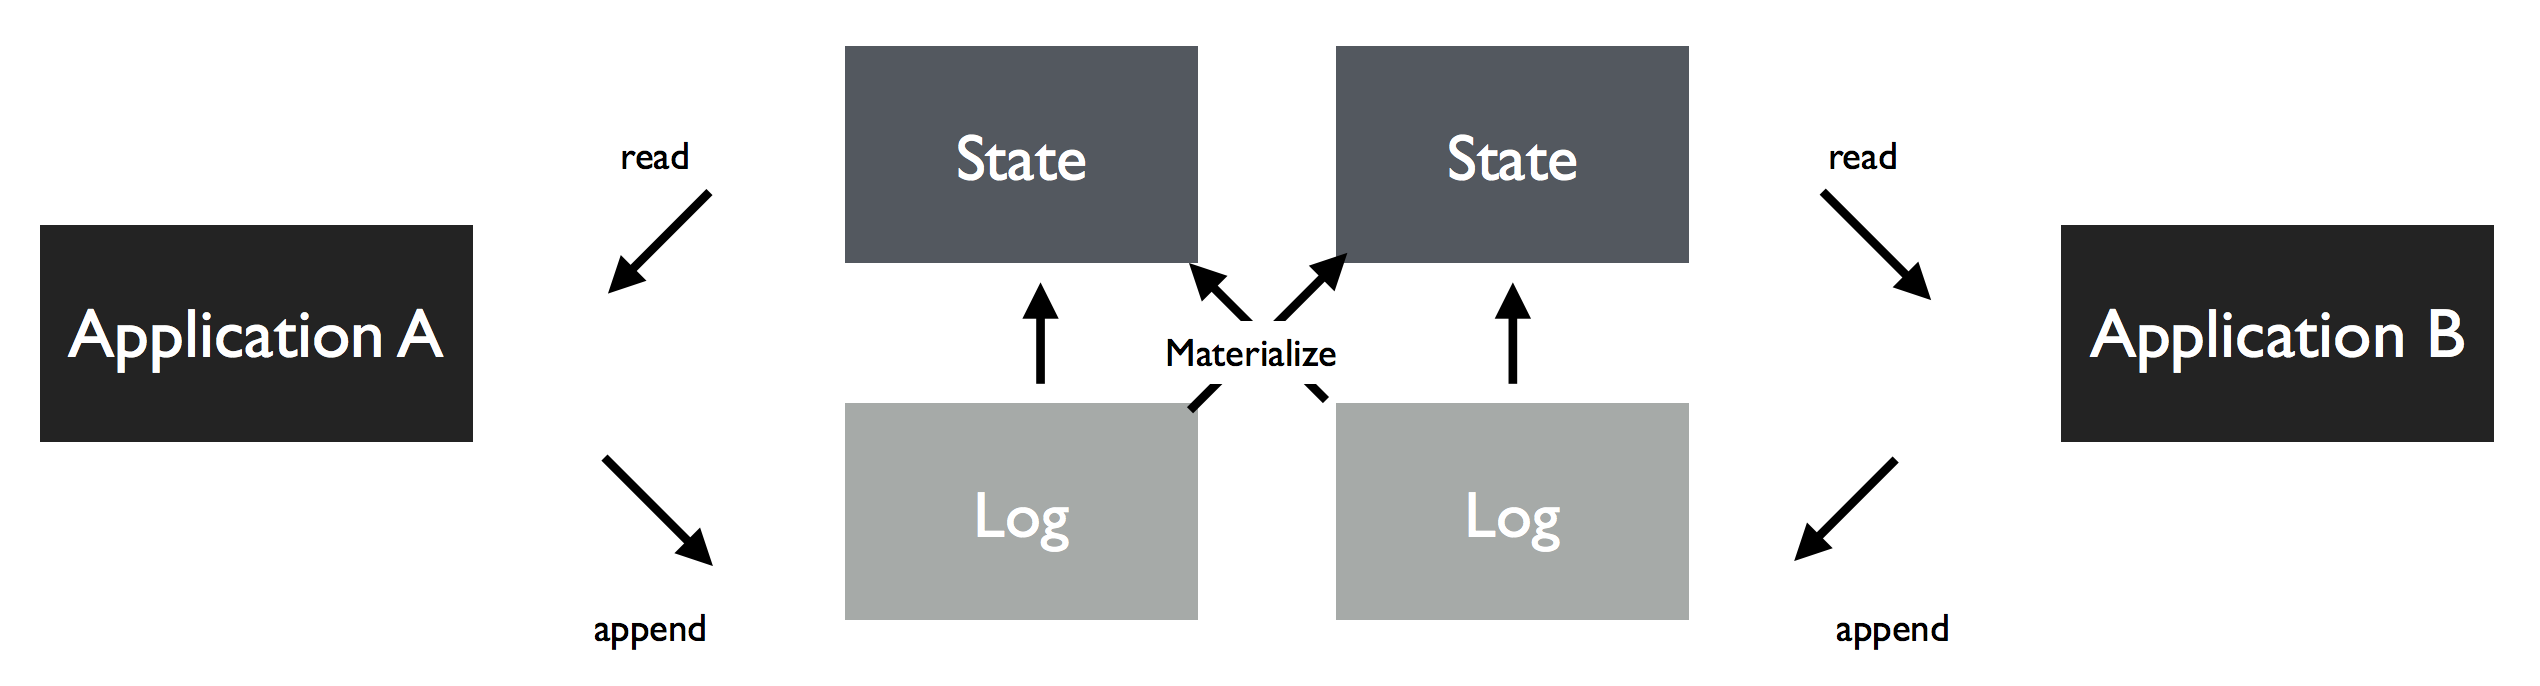
\includegraphics[width=\linewidth]{img/matstate.png}

\subsection{Lambda architecture}
Nathan Marz came up with the term Lambda Architecture (LA) for a generic, scalable and fault-tolerant data processing architecture, based on his experience working on distributed data processing systems at Backtype and Twitter.

The LA aims to satisfy the needs for a robust system that is fault-tolerant, both against hardware failures and human mistakes, being able to serve a wide range of workloads and use cases, and in which low-latency reads and updates are required. The resulting system should be linearly scalable, and it should scale out rather than up.

Here’s how it looks like, from a high-level perspective:

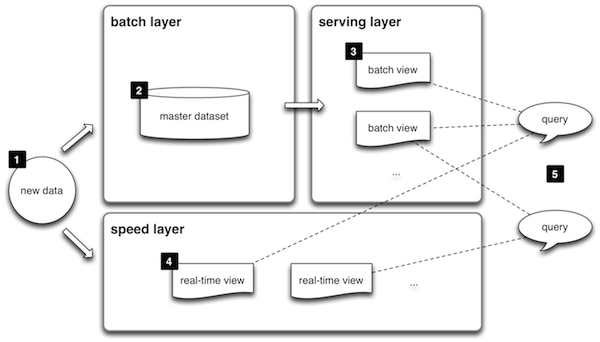
\includegraphics[width=\linewidth]{img/la-arch.png}

\begin{itemize}
\item 1. All data entering the system is dispatched to both the batch layer and the speed layer for processing.
\item 2. The batch layer has two functions: (i) managing the master dataset (an immutable, append-only set of raw data), and (ii) to pre-compute the batch views.
\item 3. The serving layer indexes the batch views so that they can be queried in low-latency, ad-hoc way.
\item 4. The speed layer compensates for the high latency of updates to the serving layer and deals with recent data only.
\item 5. Any incoming query can be answered by merging results from batch views and real-time views.
\end{itemize}

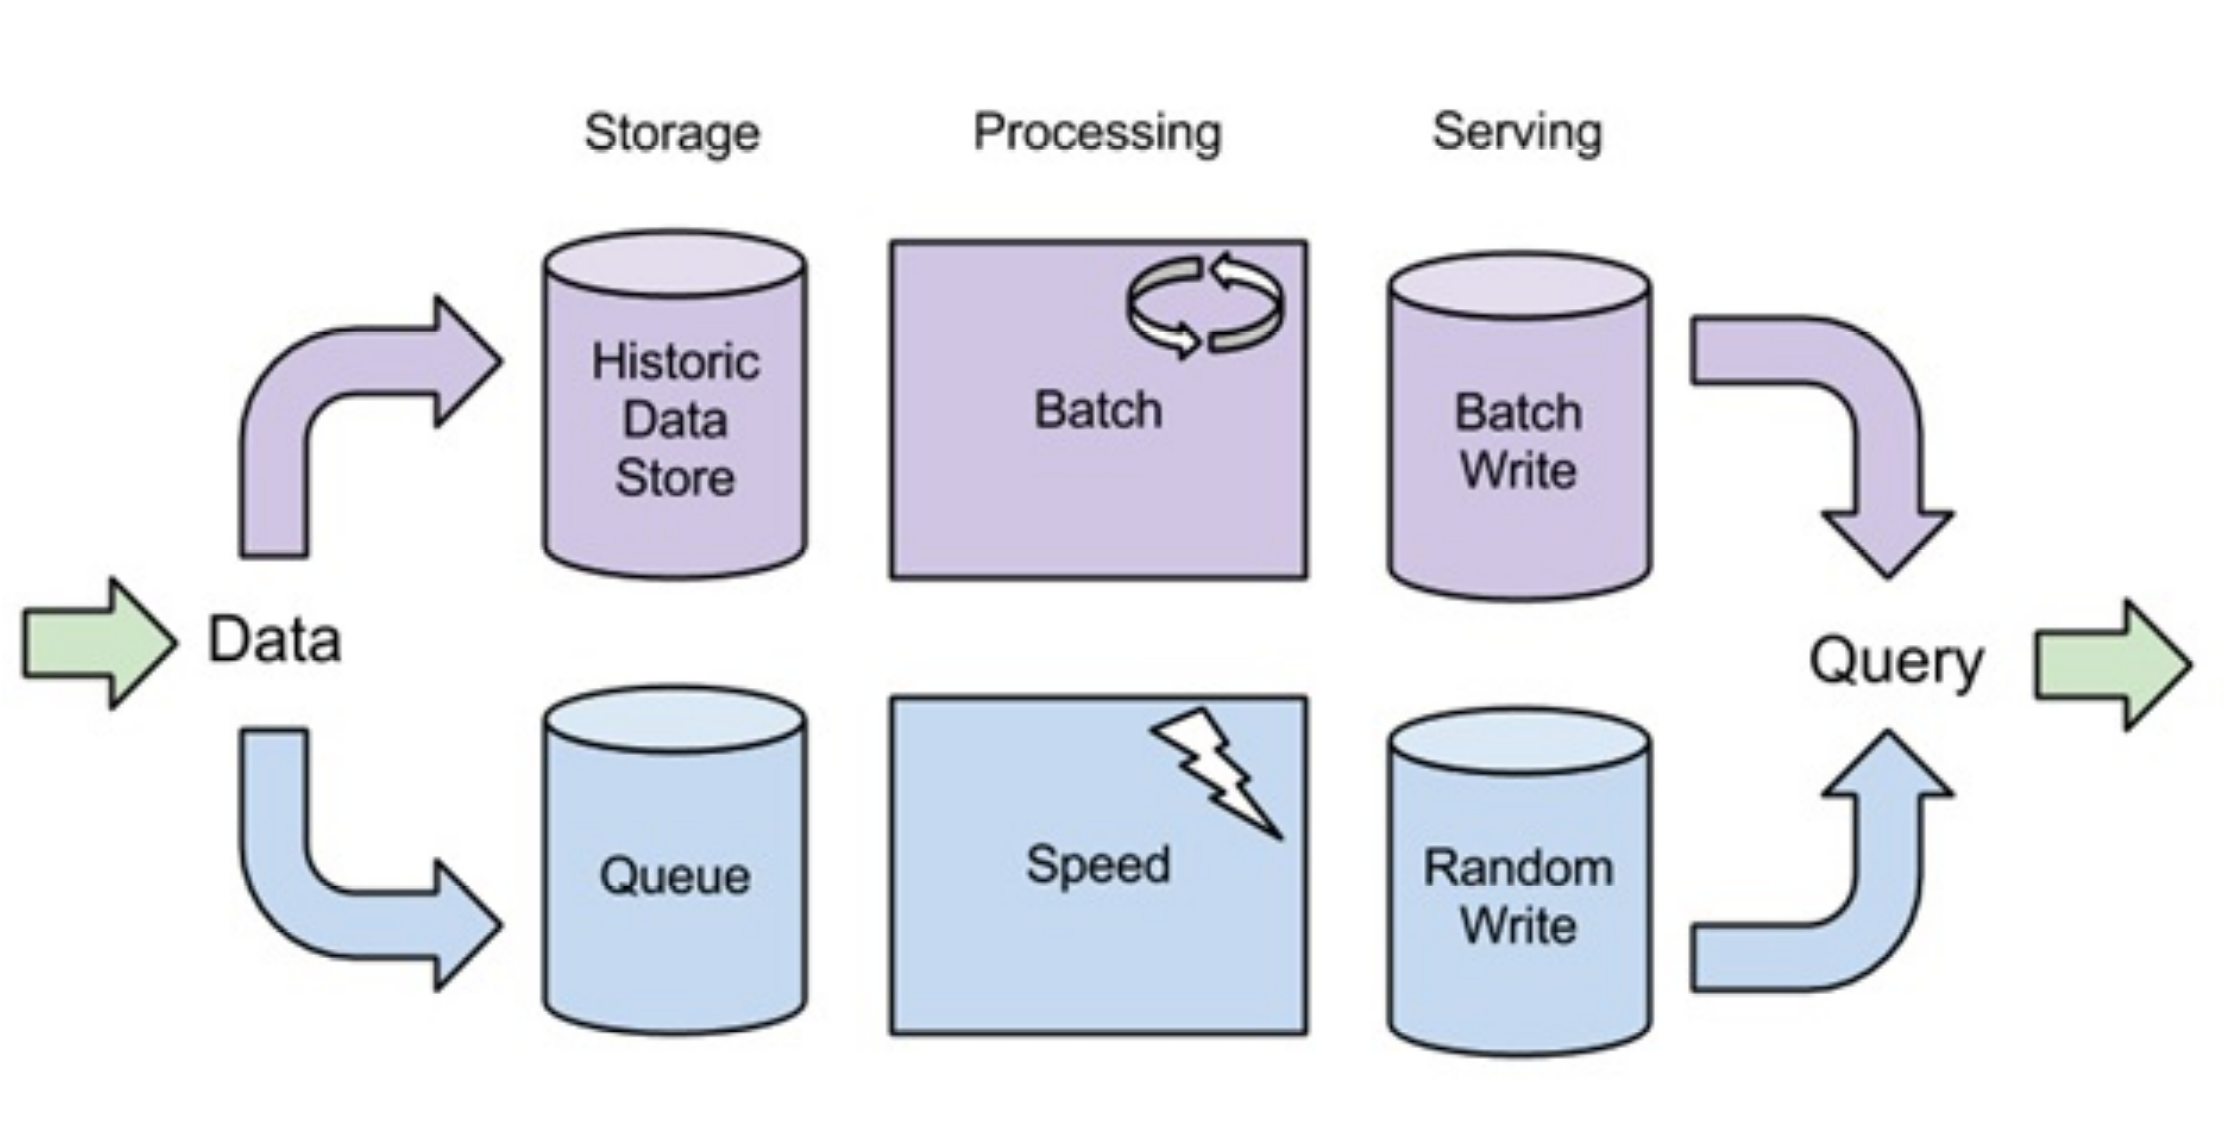
\includegraphics[width=\linewidth]{img/la-2.png}

\subsection{open questions} 
Ad blocker. ID of devices.

\subsection{Cloud Computing}
Commodity Computation, outsourced infrastructure and ability of scaling down and up on demand.


\section{Distributed Systems Coordination}
$$Agreement \Leftrightarrow Consensus \Leftrightarrow Consistency$$

\paragraph{Atomic broadcast}
\begin{itemize}
    \item Total Order property:

        $p, q$ two correct node and $m, n$ two message $\Rightarrow$ if $p$
        delivers $m$ before $n$ then $q$ delivers $m$ before $n$.

        $\rightarrow $ It's a strong consistency.

    \item No creation of message
    \item No duplication of message (delivered once)
\end{itemize}

This could be useful to have replication because all
database replicas apply updates/queries  in  
the  same  order.

\subsection{Zookeeper}
Zookeeper is a set of data node (\textbf{znodes}) which are organized in a
hierarchical namespace that resembles customary file systems. 
This file system is designed to store \textbf{metadata} and not data.
Zookeeper is a \textsc{CP} for the CAP point of view.

The \textbf{znodes} can be of two types:

\begin{itemize}
	\item \textbf{regular}: clients manipulate regular znodes by creating and deleting them explicitly.
	\item \textbf{ephemeral}: clients can delete them explicitly or let the system remove them automatically when their session terminates.
\end{itemize}

\paragraph{Session}
Client connects  to  Zookeeper  and  initiates  a  session
which allow client to move from one server to another. 
Any server can serve client's requests.

If the server fail, the client library tries to  contact  another  server
before  session  expires.

\paragraph{Consensus}
Zookeeper  can  solve  consensus  (agreement)   for  arbitrary  number  
of  clients.

\subsubsection{Global structure}
\begin{tabular}{m{8cm}m{8cm}}
    \begin{itemize}
        \item Fully replicated (no partitionning)
        \item Use commit log and periodic snapshot to recovery
            on crash
        \end{itemize}
    &
    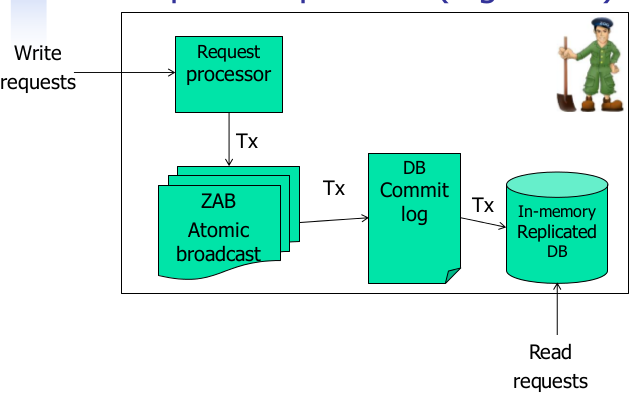
\includegraphics[width=8cm]{img/zookCompo}
\end{tabular}

\subsubsection{Operations}
Only full reads and write operations which can 
be asynchronous (concurrent calls allowed and so multiple requests) or synchronous
(no concurrent calls by a single client).

\begin{tabular}{m{9cm}m{6cm}}
    \begin{itemize}
        \item \textbf{Write}:
            \begin{tabular}{l}
                \texttt{create(znode, data, flags)}\\
                \texttt{setData(znode, data, version)}\\
                \texttt{delete(znode, version)}\\
                \texttt{sync()}
            \end{tabular}

            \paragraph{Linearizable} Write are linearizable.

            \begin{enumerate}
                \item Write request is forwarded by a follower
                    to the leader
                \item Leader use atomic (total-order) broadcast to
                    disseminate messages

                    $\rightarrow$ use ZAB protocol which support  FIFO/causal  
                    consistency  of  asynchronous  calls. 
                    ZAB tolerate $\frac{n-1}{2}$ failures.
            \end{enumerate}

            \paragraph{ZAB} use a internally elects leader for replica 
            (which is adopted by zookeeper)
            
            \paragraph{Request Processor}
            Upon receiving write request, the leader calculates in what state 
            the system will be after the write is applied and transforms the operation
            in the transactional update. These transactional update are then 
            processed by the ZAB and the DB.
            %TODO slide 64 for 11

        \item \textbf{Read}:
            \begin{tabular}{l}
                \texttt{exist(znode, watch)}\\
                \texttt{getData(znode, watch)}\\
                \texttt{getChildren(znode, watch)}
            \end{tabular}

            \paragraph{Linearizable}
            Read has \textbf{local read} (A  server  serving  a  read  request  might  not  have  been  a  part  of  a  write  
            quorum  of  some  previous  operation). 
            But if \texttt{sync()} is use before each read, we have a \textbf{linearizable read}.

            Indeed, the linearizable read is show as a \textit{slow read}.

            \paragraph{Caching reads}
    \end{itemize}
    &
    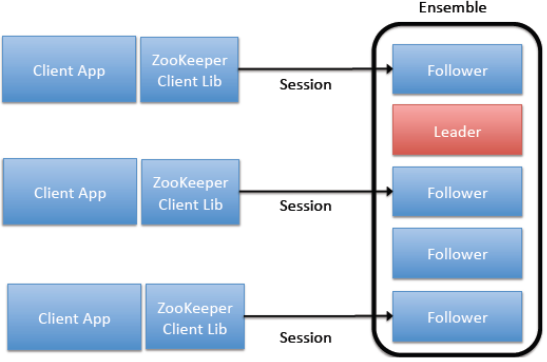
\includegraphics[width=7cm]{img/zook}
\end{tabular}

Leader atomically broadcast updates but read operations is processed
locally.


\subsubsection{Examples}
%TODO slides 51 to 59 for 11

\section{Raft}
Raft is a consensus algorithm for replicated logs which correspond to
replicated the state machine (all servers execute same commands in same order).

\begin{center}
    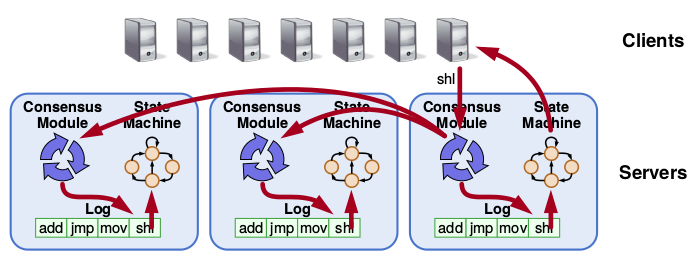
\includegraphics[width=9cm]{img/raft}
\end{center}

\subsection{Client protocol}
Client send command to leader (or other server that will redirect
to leader) and the leader does not respond until command as been
(1) logged, (2) committed and (3) executed by leader's state machine.

\paragraph{Unique ID} has use to identify a client command and has store in
log. This allow to not execute a command twice if leader crashes after
executing command, but before responding.

\subsection{Overview}

\subsubsection{Consensus}
Consensus is leader-based which is more efficient thant leader-less approach
and allow to simplifies normal operation because there is no conflict.

\subsubsection{Server states}

\begin{itemize}
    \item At any given time, each servier is EITHER :
        \begin{enumerate}
            \item Follower : completely passive 
            \item Candidate : used to elect a new leader
            \item Leader: handles all client interactions, log replication
        \end{enumerate}
    \item Time divided into term (maintains current term value)
\end{itemize}

\begin{center}
    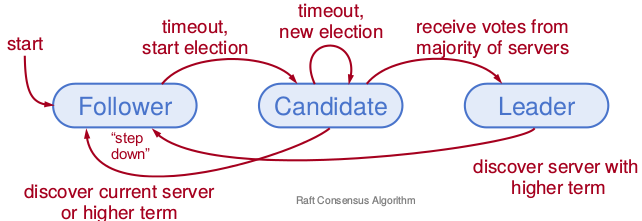
\includegraphics[width=9cm]{img/rleader}
\end{center}

\subsubsection{Terms}
\begin{tabular}{m{8cm}m{6cm}}
    Time divided into term
    \begin{itemize}
        \item at most one leader per term
        \item If no leader on term then failed election
    \end{itemize}
    Term is used to identify obsolete information
    &
    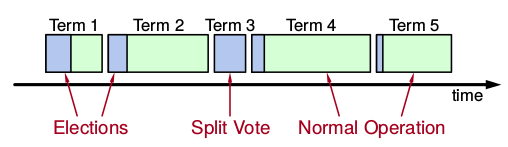
\includegraphics[width=9cm]{img/term}
\end{tabular}

As every RPC contain term of send, \textbf{terms} are used to detect stale
leaders (and candidates) because each election increment the term counter.
\begin{itemize}
    \item If sender’s term is older, RPC is rejected, sender reverts to
        follower and updates its term
    \item if receiver’s term is older, it reverts to follower, updates its term,
        then processes RPC normally
\end{itemize}

\subsubsection{Heartbeats}
\begin{itemize}
    \item Servers start up as followers
    \item Followers expect to receive RPCs from leader or candidates
    \item Leader must send heartbeats (empty
        AppendEntries RPCs) to maintain authority.

        \texttt{ElectionTimeout} without receive RPCs $\rightarrow$ assume that
        leader has crashed.
\end{itemize}


\subsubsection{Leader election}

\begin{enumerate}
    \item Increment current term
    \item Change to candidate state
    \item Vote for self
    \item Send \texttt{Request Vote RPC} (which include
        index and term of last log entry) to all other server
        \begin{itemize}
            \item Receive vote from majority $\Rightarrow$ leader
            \item Receive RPC from valid leader $\Rightarrow$ follower state
            \item Election timeout elapse $\Rightarrow$ new election
        \end{itemize}
\end{enumerate}

Note that the candidate is choose in order to have the leader
with the most complete log.

\begin{itemize}
    \item \textbf{Safety}: allow at most one winner per term because
        each server gives only one vote per term and it's impossible two
        have two different candidates with majorities of vote.

    \item \textbf{Liveness}: some candidate must eventually win.

        $T \leq$ Election timeouts $\leq 2T$, so usually one server
        timeout and wins elections before other wake up.
        (Work well if $T >>$ broadcast time)
\end{itemize}

\subsubsection{Normal operation}
\begin{enumerate}
    \item Client sends command to leader
    \item Leader appends command to its log
    \item Leader sends AppendEntries RPCs to followers
    \item Once new entry committed:
        \begin{enumerate}
            \item  Leader passes command to its state machine, returns result to
                client
            \item  Leader notifies followers of committed entries in subsequent
                AppendEntries RPCs
            \item  Followers pass committed commands to their state machines
        \end{enumerate}
\end{enumerate}

If there is crashed/slow followers,
Leader retries RPCs until they succeed.

$\rightarrow$  Performance is optimal if one successful RPC to any majority of
servers.

\subsection{Log}

\subsubsection{Structure}

\begin{tabular}{m{6cm}m{8cm}}
    Leader take commands from clients and replicates its log to other server.
    \begin{itemize}
        \item Entry \textbf{committed} if know to be stored on majority of servers
    \end{itemize}
    Term is used to identify obsolete information
    &
    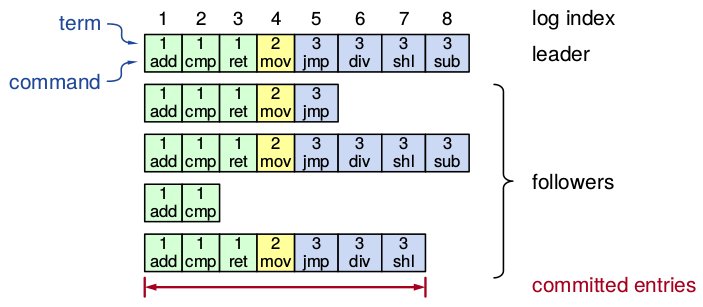
\includegraphics[width=11cm]{img/raftLog}
\end{tabular}

\subsubsection{Consistency}
\begin{itemize}
    \item If log entries on different servers have same index
        and term then (1) they store the same command and (2) the logs are identical
        in all preceding entries
    \item If a given entry is committed, all preceding entries are also committed
\end{itemize}

\subsubsection{Safety}
Raft safety property say that if a leader has decided that a log entry is committed, that entry
will be present in the logs of all future leaders.

To guarantee the safety requirement:
\begin{itemize}
    \item Leaders never overwrite entries in their logs
    \item Only entries in the leader’s log can be committed
    \item Entries must be committed before applying to state machine
\end{itemize}

\subsubsection{Append entries}
Each \texttt{AppendEntries RPC} contains index and term of entry preceding new
ones. This entry must match before append the new entry.

\subsubsection{Commitment rules}
If a leader decide to commit an entry:
\begin{enumerate}
    \item this entry must be stored on a majority of server
    \item \textbf{AND} at least one new entry from leader's term must 
        also be stored on majority of servers
\end{enumerate}

\begin{center}
\begin{tabular}{m{7cm}cm{7cm}}
    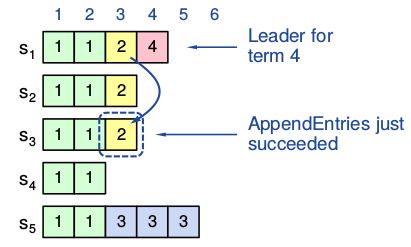
\includegraphics[width=7cm]{img/commitFault}
    &
    $\Rightarrow$
    &
    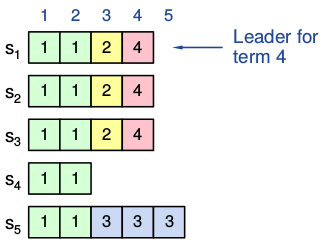
\includegraphics[width=6cm]{img/commitRight}
    \\
    Not safe commit for previous term because $s_5$ can
    be the next leader. (Without 2. commitment rules)
    & &
    Safe commit because $s_5$ cannot be the next leader
    (With 2. commitment rules) \\
\end{tabular}
\end{center}


\subsubsection{Repairing follower logs}
Leader must make follower logs consistent with its own
by (1) delete extraneous entries and (2) fill in missing entries.

\begin{tabular}{m{6cm}m{8cm}}
    \begin{itemize}
        \item Leader keep \textbf{nextIndex} for each follower (initialized
            to $1+leaderIndex$)
        \item When AppendEntries consistency check fails, decrement
            nextIndex and try again
        \item Not that when follower overwrites inconsistent entry, it
            deletes all next entries
    \end{itemize}
    &
    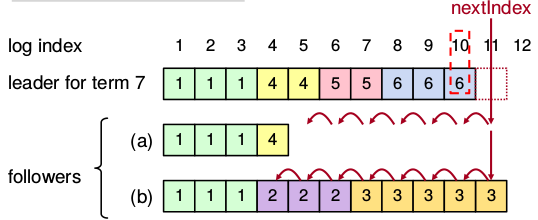
\includegraphics[width=11cm]{img/repairing}
\end{tabular}

\subsection{Configuration}
%TODO slide 27-28-29-30 for 12

\section{Notes on summaries}

These summaries are nearly just copy/pasted from the original papers. They allow you to save time by only taking essentials.

\section{Summary of The Google File System (GFS)}

\subsection{Design overview : Assumptions}

\begin{itemize}
\item It must constantly monitor
itself and detect, tolerate, and \textbf{recover promptly from
component failures on a routine basis}.
\item The system stores a modest number of large files. We
expect a few million files, each typically 100 MB or
larger in size. Multi-GB files are the common case
and should be managed efficiently. \textbf{Small files must be
supported, but we need not optimize for them.}
\item The workloads primarily consist of two kinds of reads:
\textbf{large streaming reads and small random reads}. In
large streaming reads, individual operations typically
read hundreds of KBs, more commonly 1 MB or more.
Successive operations from the same client often read
through a contiguous region of a file. A small random
read typically reads a few KBs at some arbitrary
offset. Performance-conscious applications often batch
and sort their small reads to advance steadily through
the file rather than go backand forth.
\item The workloads also have many large, sequential writes
that append data to files. Typical operation sizes are
similar to those for reads. Once written, files are seldom
modified again. \textbf{Small writes at arbitrary positions
in a file are supported but do not have to be
efficient.}
\item The system must efficiently implement well-defined semantics
for multiple clients that concurrently append
to the same file. Our files are often used as producerconsumer
queues or for many-way merging. \textbf{Hundreds
of producers, running one per machine, will concurrently
append to a file}. Atomicity with minimal synchronization
overhead is essential. The file may be
read later, or a consumer may be reading through the
file simultaneously.
\item \textbf{High sustained bandwidth is more important than low
latency}. Most of our target applications place a premium
on processing data in bulkat a high rate, while
few have stringent response time requirements for an
individual read or write
\end{itemize}

We support the usual operations to \textbf{create, delete,
open, close, read, and write files}.
Moreover, GFS has \textbf{snapshot and record append operations}.
Snapshot creates a copy of a file or a directory tree
at low cost. Record append allows multiple clients to \textbf{append
data to the same file concurrently while guaranteeing
the atomicity of each individual client’s append}.

\subsection{Architecture}

A GFS cluster consists of a single master and multiple
chunkservers and is accessed by multiple clients.

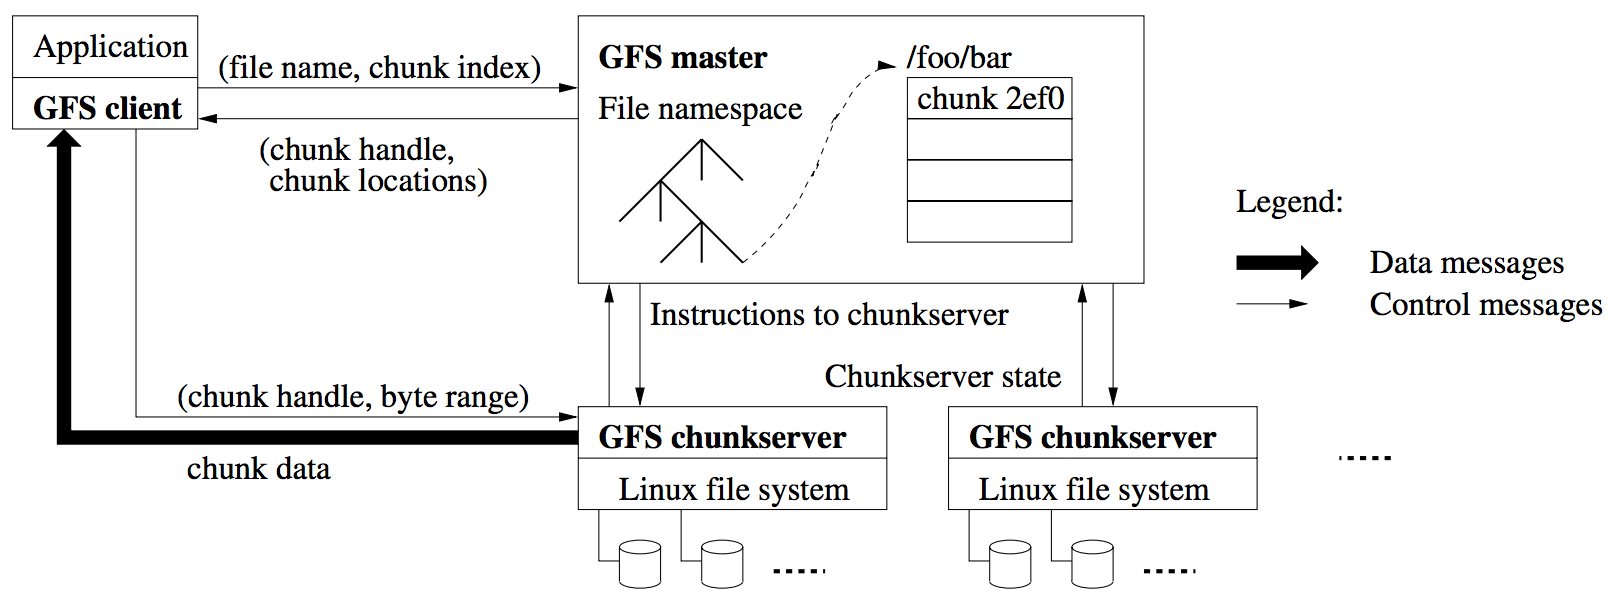
\includegraphics[width=\linewidth]{img/gfs.png}

Files are divided into fixed-size chunks. Each chunkis
identified by an immutable and globally unique 64 bit chunk
handle assigned by the master at the time of chunkcreation.
Chunkservers store chunks on local disks as Linux files and
read or write chunkdata specified by a chunkhandle and
byte range. For reliability, each chunkis replicated on multiple
chunkservers. By default, we store three replicas, though
users can designate different replication levels for different
regions of the file namespace.

The master maintains all file system metadata. This includes
the namespace, access control information, the mapping
from files to chunks, and the current locations of chunks.
It also controls system-wide activities such as chunklease
management, garbage collection of orphaned chunks, and
chunkmigration between chunkservers. The master periodically
communicates with each chunkserver in HeartBeat
messages to give it instructions and collect its state.

Clients interact with the master for metadata operations,
but all data-bearing communication goes directly to
the chunkservers.

Neither the client nor the chunkserver caches file data.
Client caches offer little benefit because most applications
stream through huge files or have working sets too large
to be cached. Not having them simplifies the client and
the overall system by eliminating cache coherence issues.
(Clients do cache metadata, however.) Chunkservers need
not cache file data because chunks are stored as local files
and so Linux’s buffer cache already keeps frequently accessed
data in memory.


\subsection{Single master}

The client typically asks for multiple chunks in the
same request and the master can also include the information
for chunks immediately following those requested. This
extra information sidesteps several future client-master interactions
at practically no extra cost. The client uses a cache for these metadata. 

\subsection{Chunk Size}

Chunksize is one of the key design parameters. We have
chosen 64 MB, which is much larger than typical file system
blocksizes. Each chunkreplica is stored as a plain
Linux file on a chunkserver and is extended only as needed.
Lazy space allocation avoids wasting space due to internal
fragmentation, perhaps the greatest objection against such
a large chunksize.

A large chunksize offers several important advantages.
First, it reduces clients’ need to interact with the master
because reads and writes on the same chunkrequire only
one initial request to the master for chunklocation information.
The reduction is especially significant for our workloads
because applications mostly read and write large files
sequentially. Even for small random reads, the client can
comfortably cache all the chunklocation information for a
multi-TB working set. Second, since on a large chunk, a
client is more likely to perform many operations on a given
chunk, it can reduce network overhead by keeping a persistent
TCP connection to the chunkserver over an extended
period of time. Third, it reduces the size of the metadata
stored on the master. This allows us to keep the metadata
in memory.

\textbf{A large chunksize, even with lazy space
allocation, has its disadvantages}.  A small file consists of a
small number of chunks, \textbf{perhaps just one}. The chunkservers
storing those chunks may become \textbf{hot spots if many clients
are accessing the same file}. In practice, hot spots have not
been a major issue because our applications mostly read
large multi-chunkfiles sequentially.

Hot spots did develop when GFS was first used
by a batch-queue system: \textbf{an executable was written to GFS
as a single-chunkfile and then started on hundreds of machines
at the same time}. The few chunkservers storing this
executable were overloaded by hundreds of simultaneous requests.
We fixed this problem by storing such executables
with a higher replication factor and by making the batchqueue
system stagger application start times. A potential
long-term solution is to allow clients to read data from other
clients in such situations.

\subsection{Metadata}

Three major types of metadata:
\begin{description}
\item[the file and chunknamespaces]
\item[the mapping from files to chunks]
\item[the locations of each chunk’s replicas] The master does not store chunklocation information persistently. Instead, it asks each chunkserver about its chunks at master startup and whenever a chunkserver joins the cluster.
\end{description}

The first two types (namespaces
and file-to-chunkmapping) are also kept persistent by
logging mutations to an operation log stored on the master’s
local diskand replicated on remote machines. Using
a log allows us to update the master state simply, reliably,
and without risking inconsistencies in the event of a master
crash.

\subsubsection{In-Memory Data Structures}

Since metadata is stored in memory, master operations are
fast. Furthermore, it is easy and efficient for the master to
periodically scan through its entire state in the background.
This periodic scanning is used to implement chunkgarbage
collection, re-replication in the presence of chunkserver failures,
and chunkmigration to balance load and diskspace usage across chunkservers.

One potential concern for this memory-only approach is
that the number of chunks and hence the capacity of the
whole system is limited by how much memory the master
has.  The cost of adding extra memory to the master is a small price to pay
for the simplicity, reliability, performance, and flexibility we
gain by storing the metadata in memory.

\subsubsection{Chunk Locations}

\textbf{The master does not keep a persistent record of which
chunkservers have a replica of a given chunk. It simply polls
chunkservers for that information at startup}. The master
can keep itself up-to-date thereafter because it controls all
chunkplacement and monitors chunkserver status with regular
HeartBeat messages.

\subsubsection{Operation Log}

The operation log contains a historical record of critical
metadata changes.

Files and chunks, as well as their versions are all uniquely and eternally identified by the logical times at which they were created.

Since the operation log is critical, \textbf{we must store it reliably
and not make changes visible to clients until metadata
changes are made persistent}. Otherwise, we effectively lose
the whole file system or recent client operations even if the
chunks themselves survive. Therefore, we replicate it on
multiple remote machines and respond to a client operation
only after flushing the corresponding log record to disk
both locally and remotely. The master batches several log
records together before flushing thereby reducing the impact
of flushing and replication on overall system throughput.

The master recovers its file system state by replaying the
operation log. To minimize startup time, we must keep the
log small.  GFS uses checkpoints to do so. The new checkpoint
includes all mutations before the switch. It can be created
in a minute or so for a cluster with a few million files. When
completed, it is written to diskboth locally and remotely.

\subsection{Consistency Model}

File namespace mutations (e.g., file creation) are atomic.
They are handled exclusively by the master: namespace
locking guarantees atomicity and correctness. The master’s operation log defines a global total order of these operations.

\textbf{A file region is consistent if all clients will
always see the same data, regardless of which replicas they
read from}. A region is defined after a file data mutation if it
is consistent and clients will see what the mutation writes in
its entirety. When a mutation succeeds without interference
from concurrent writers, the affected region is defined (and
by implication consistent): all clients will always see what
the mutation has written. \textbf{Concurrent successful mutations
leave the region undefined but consistent: all clients see the
same data, but it may not reflect what any one mutation
has written}.

Data mutations may be \textbf{writes} or \textbf{record appends}. \textbf{A write
causes data to be written at an \underline{application-specified file
offset}}. \textbf{A record append causes data (the “record”) to be
appended atomically at least once even in the presence of
concurrent mutations, but at \underline{an offset of GFS’s choosing}}. The offset is returned to the client and marks
the beginning of a defined region that contains the record.
In addition, GFS may insert padding or record duplicates in
between. They occupy regions considered to be inconsistent
and are typically dwarfed by the amount of user data.

\begin{figure}[!h]
\centering
\includegraphics[width=0.6\linewidth]{img/summary_consistency_gfs.png}
\end{figure}

After a sequence of successful mutations, the mutated file
region is guaranteed to be defined and contain the data written
by the last mutation. GFS achieves this by
\begin{itemize}
\item applying
mutations to a chunkin the same order on all its replicas
\item using chunkversion numbers to detect
any replica that has become stale because it has missed mutations
while its chunkserver was down
\end{itemize}

Stale replicas will never be involved in a mutation or given to
clients asking the master for chunk locations. They are
garbage collected at the earliest opportunity.

Since clients cache chunklocations, they may read from a
stale replica before that information is refreshed. This window
is limited by the cache entry’s timeout and the next
open of the file, which purges from the cache all chunkinformation
for that file. Moreover, as most of our files are
append-only, a stale replica usually returns a premature
end of chunkrather than outdated data. When a reader
retries and contacts the master, it will immediately get current
chunklocations.

Long after a successful mutation, component failures can
of course still corrupt or destroy data. GFS identifies failed
chunkservers by regular handshakes between master and all
chunkservers and \textbf{detects data corruption by checksumming}.

A chunk is lost irreversibly only if all its replicas are lost before GFS
can react, typically within minutes. Even in this case, it becomes
unavailable, not corrupted: applications receive clear
errors rather than corrupt data.

\subsubsection{Implications for Applications}

GFS applications can accommodate the relaxed consistency
model with a few simple techniques already needed for
other purposes: relying on appends rather than overwrites,
checkpointing, and writing self-validating, self-identifying
records.

Practically all our applications \textbf{mutate files by appending
rather than overwriting}.

In the other typical use, many writers concurrently append
to a file for merged results or as a producer-consumer
queue. Record append’s append-at-least-once semantics preserves
each writer’s output. Readers deal with the occasional
padding and duplicates as follows. \textbf{Each record prepared
by the writer contains extra information like \underline{checksums}
so that its validity can be verified. A reader can
identify and discard extra padding and record fragments
using the checksums}. If it cannot tolerate the occasional
duplicates (e.g., if they would trigger non-idempotent operations),
\textbf{it can \underline{filter them out} using unique identifiers in
the records, which are often needed anyway to name corresponding
application entities such as web documents}. These
functionalities for record I/O (except duplicate removal) are
in library code shared by our applications and applicable to
other file interface implementations at Google. With that,
the same sequence of records, plus rare duplicates, is always
delivered to the record reader.

\subsection{Leases and Mutation Order}

We use leases to \textbf{maintain a consistent mutation order across
replicas}. The master grants a chunklease to one of the replicas,
which we call the primary. The primary picks a serial
order for all mutations to the chunk. All replicas follow this
order when applying mutations. Thus, the global mutation
order is defined first by the lease grant order chosen by the
master, and within a lease by the serial numbers assigned
by the primary.

The lease mechanism is designed to minimize management
overhead at the master. A lease has an initial timeout
of 60 seconds. However, as long as the chunkis being mutated,
the primary can request and typically receive extensions
from the master indefinitely. These extension requests
and grants are piggybacked on the HeartBeat messages regularly
exchanged between the master and all chunkservers.
The master may sometimes try to revoke a lease before it
expires (e.g., when the master wants to disable mutations
on a file that is being renamed). Even if the master loses
communication with a primary, it can safely grant a new
lease to another replica after the old lease expires.

\begin{figure}[!h]
\centering
\includegraphics[width=0.6\linewidth]{img/gfs_data_control.png}
\end{figure}

Once a chunkserver receives some data, it starts forwarding immediately.
Control and data flows are decoupled.

\subsection{Snapshot}

we use standard copy-on-write techniques to
implement snapshots. When the master receives a snapshot
request, it first revokes any outstanding leases on the chunks
in the files it is about to snapshot. This ensures that any
subsequent writes to these chunks will require an interaction
with the master to find the lease holder. This will give the
master an opportunity to create a new copy of the chunk
first.

By creating the new chunkon the same chunkservers as the original, we
ensure that the data can be copied locally, not over the network(our
disks are about three times as fast as our 100 Mb
Ethernet links).

\section{Summary of Amazon’s Highly Available Key-value Store}

This paper presents the design and implementation of Dynamo, another highly available and scalable distributed data store built for Amazon’s platform. 

Using a relational database would lead to inefficiencies and limit scale and availability.

Dynamo uses a synthesis of well known techniques to achieve
scalability and availability: Data is partitioned and replicated
using consistent hashing [10], and consistency is facilitated by
object versioning [12]. The consistency among replicas during
updates is maintained by a quorum-like technique and a
decentralized replica synchronization protocol. 
Dynamo employs a gossip (reports about other people, typically involving details that are not confirmed as being true) based distributed failure detection and membership protocol. Dynamo is a completely decentralized system with
minimal need for manual administration. Storage nodes can be
added and removed from Dynamo without requiring any manual
partitioning or redistribution. 

\subsection{System Assumptions and Requirements}

\begin{itemize}
\item[Query Model] simple read and write operations to a data item that
is uniquely identified by a key. State is stored as binary objects
(i.e., blobs) identified by unique keys. No operations span
multiple data items and there is no need for relational schema. 

\item[ACID Properties] ACID (Atomicity, Consistency, Isolation,
Durability) is a set of properties that guarantee that database
transactions are processed reliably. In the context of databases, a
single logical operation on the data is called a transaction.
Experience at Amazon has shown that data stores that provide
ACID guarantees tend to have poor availability. Dynamo targets applications that operate with weaker consistency
(the “C” in ACID) if this results in high availability. Dynamo
does not provide any isolation guarantees and permits only single
key updates. 

\item[Efficiency] response within 300ms for 99.9\% of its requests for a
peak client load of 500 requests per second.

\item[Other Assumptions] Dynamo is used only by Amazon’s internal
services. Its operation environment is assumed to be non-hostile
and there are no security related requirements such as
authentication and authorization.
\end{itemize}

\subsection{Design considerations : Resolution on read, not write}
An important design consideration is to decide when to perform
the process of resolving update conflicts, i.e., whether conflicts
should be resolved during reads or writes. Many traditional data
stores execute conflict resolution during writes and keep the read
complexity simple [7]. In such systems, writes may be rejected if
the data store cannot reach all (or a majority of) the replicas at a
given time. On the other hand, Dynamo targets the design space
of an “always writeable” data store (i.e., a data store that is highly
available for writes). For a number of Amazon services, rejecting
customer updates could result in a poor customer experience. For
instance, the shopping cart service must allow customers to add
and remove items from their shopping cart even amidst network
and server failures. This requirement forces us to push the
complexity of conflict resolution to the reads in order to ensure
that writes are never rejected. 

The next design choice is who performs the process of conflict
resolution. This can be done by the data store or the application. If
conflict resolution is done by the data store, its choices are rather
limited. In such cases, the data store can only use simple policies,
such as “last write wins” [22], to resolve conflicting updates. On
the other hand, since the application is aware of the data schema it
can decide on the conflict resolution method that is best suited for
its client’s experience. For instance, the application that maintains
customer shopping carts can choose to “merge” the conflicting
versions and return a single unified shopping cart. Despite this
flexibility, some application developers may not want to write
their own conflict resolution mechanisms and choose to push it
down to the data store, which in turn chooses a simple policy such
as “last write wins”. 

\begin{description}
\item[Incremental scalability] Dynamo should be able to scale out one
storage host (henceforth, referred to as “node”) at a time, with
minimal impact on both operators of the system and the system
itself.

\item[Symmetry] Every node in Dynamo should have the same set of
responsibilities as its peers; there should be no distinguished node
or nodes that take special roles or extra set of responsibilities. In
our experience, symmetry simplifies the process of system
provisioning and maintenance

\item[Decentralization] An extension of symmetry, the design should
favor decentralized peer-to-peer techniques over centralized
control. In the past, centralized control has resulted in outages and
the goal is to avoid it as much as possible. This leads to a simpler,
more scalable, and more available system.

\item[Heterogeneity] The system needs to be able to exploit
heterogeneity in the infrastructure it runs on. e.g. the work
distribution must be proportional to the capabilities of the
individual servers. This is essential in adding new nodes with
higher capacity without having to upgrade all hosts at once.

\end{description}

\subsection{techniques used by Dynamo}

\begin{tabular}{p{4.5cm}|p{4.5cm}|p{4.5cm}}
Problem & Technique & Advantage \\
\hline
\hline
Partitioning & Consistent Hashing  & Incremental + Scalability \\
\hline
High Availability for writes  & Vector clocks with reconciliation during reads & Version size is decoupled from update rates. \\  
\hline
Handling temporary
failures  & Sloppy Quorum and
hinted handoff & Provides high
availability and
durability guarantee
when some of the
replicas are not
available.  \\
\hline
Recovering from
permanent failures & Anti-entropy using
Merkle trees & Synchronizes
divergent replicas in
the background. \\
\hline
Membership and
failure detection  & Gossip-based
membership protocol
and failure detection. & Preserves symmetry
and avoids having a
centralized registry
for storing
membership and
node liveness
information. \\
\hline 
\end{tabular}

Dynamo treats both the key and the object supplied by the caller
as an opaque array of bytes. It applies a MD5 hash on the key to
generate a 128-bit identifier, which is used to determine the
storage nodes that are responsible for serving the key. 

\subsubsection{Scale of hashing}

Each node in the
system is assigned a random value within this space which
represents its “position” on the ring. Each data item identified by
a key is assigned to a node by hashing the data item’s key to yield
its position on the ring, and then walking the ring clockwise to
find the first node with a position larger than the item’s position. 

Thus, each node becomes responsible for the region in the ring
between it and its predecessor node on the ring. The principle
advantage of consistent hashing is that departure or arrival of a
node only affects its immediate neighbors and other nodes remain
unaffected. 

Instead of mapping a node to a single point in the circle, each node gets
assigned to multiple points in the ring. To this end, Dynamo uses
the concept of “virtual nodes”. A virtual node looks like a single
node in the system, but each node can be responsible for more
than one virtual node. Effectively, when a new node is added to
the system, it is assigned multiple positions (henceforth, “tokens”)
in the ring. 

Advantage of this system :

\begin{itemize}
\item If a node becomes unavailable (due to failures or routine
maintenance), the load handled by this node is evenly
dispersed across the remaining available nodes. 
\item When a node becomes available again, or a new node is
added to the system, the newly available node accepts a
roughly equivalent amount of load from each of the other
available nodes. 
\item The number of virtual nodes that a node is responsible can
decided based on its capacity, accounting for heterogeneity
in the physical infrastructure.
\end{itemize}

\subsubsection{Replication}

To achieve high availability and durability, Dynamo replicates its
data on multiple hosts. Each data item is replicated at N hosts,
where N is a parameter configured “per-instance”. Each key, k, is
assigned to a coordinator node (described in the previous section).
The coordinator is in charge of the replication of the data items
that fall within its range. In addition to locally storing each key
within its range, the coordinator replicates these keys at the N-1
clockwise successor nodes in the ring. This results in a system
where each node is responsible for the region of the ring between
it and its Nth predecessor. In Figure 2, node B replicates the key k
at nodes C and D in addition to storing it locally. Node D will
store the keys that fall in the ranges (A, B], (B, C], and (C, D]. 

\includegraphics[width=0.5\linewidth]{img/dynamo.png}

The list of nodes that is responsible for storing a particular key is
called the preference list

\subsubsection{Data Versioning}

Dynamo provides eventual consistency, which allows for updates
to be propagated to all replicas asynchronously. 

Dynamo uses vector clocks [12] in order to capture causality
between different versions of the same object. A vector clock is
effectively a list of (node, counter) pairs. One vector clock is
associated with every version of every object. One can determine
whether two versions of an object are on parallel branches or have
a causal ordering, by examine their vector clocks. If the counters
on the first object’s clock are less-than-or-equal to all of the nodes
in the second clock, then the first is an ancestor of the second and
can be forgotten. Otherwise, the two changes are considered to be
in conflict and require reconciliation. 

\includegraphics[width=0.5\linewidth]{img/vector_clocks.png}

In Dynamo, when a client wishes to update an object, it must
specify which version it is updating. This is done by passing the
context it obtained from an earlier read operation, which contains
the vector clock information. Upon processing a read request, if 
Dynamo has access to multiple branches that cannot be
syntactically reconciled, it will return all the objects at the leaves,
with the corresponding version information in the context. An
update using this context is considered to have reconciled the
divergent versions and the branches are collapsed into a single
new version.

It is desirable to limit the size of vector clock. To this
end, Dynamo employs the following clock truncation scheme:
Along with each (node, counter) pair, Dynamo stores a timestamp
that indicates the last time the node updated the data item. When
the number of (node, counter) pairs in the vector clock reaches a
threshold (say 10), the oldest pair is removed from the clock.
Clearly, this truncation scheme can lead to inefficiencies in
reconciliation as the descendant relationships cannot be derived
accurately. However, this problem has not surfaced in production
and therefore this issue has not been thoroughly investigated. 

\subsubsection{API interface}

get(K), put(K, X), put(K, C, X). K = key. X = content. C = context (for update).

To maintain consistency among its replicas, Dynamo uses a
consistency protocol similar to those used in quorum systems.
This protocol has two key configurable values: R and W. R is the
minimum number of nodes that must participate in a successful
read operation. W is the minimum number of nodes that must
participate in a successful write operation. Setting R and W such
that R + W > N yields a quorum-like system. In this model, the
latency of a get (or put) operation is dictated by the slowest of the
R (or W) replicas. For this reason, R and W are usually
configured to be less than N, to provide better latency. 

A node handling a read or write operation is known as the
coordinator. Typically, this is the first among the top N nodes in
the preference list. If the requests are received through a load
balancer, requests to access a key may be routed to any random
node in the ring. In this scenario, the node that receives the
request will not coordinate it if the node is not in the top N of the
requested key’s preference list. Instead, that node will forward the
request to the first among the top N nodes in the preference list. 

Upon receiving a put() request for a key, the coordinator generates
the vector clock for the new version and writes the new version
locally. The coordinator then sends the new version (along with the new vector clock) to the N highest-ranked reachable nodes. If
at least W-1 nodes respond then the write is considered
successful. 

Similarly, for a get() request, the coordinator requests all existing
versions of data for that key from the N highest-ranked reachable
nodes in the preference list for that key, and then waits for R
responses before returning the result to the client. If the
coordinator ends up gathering multiple versions of the data, it
returns all the versions it deems to be causally unrelated. The
divergent versions are then reconciled and the reconciled version
superseding the current versions is written back. 


\subsubsection{Handling Failures: Hinted Handoff}

It uses a “sloppy quorum”; all read and
write operations are performed on the first N healthy nodes from
the preference list, which may not always be the first N nodes
encountered while walking the consistent hashing ring. 

Consider the example of Dynamo configuration given in Figure 2
with N=3. In this example, if node A is temporarily down or
unreachable during a write operation then a replica that would
normally have lived on A will now be sent to node D. This is done
to maintain the desired availability and durability guarantees. The
replica sent to D will have a hint in its metadata that suggests
which node was the intended recipient of the replica (in this case
A). Nodes that receive hinted replicas will keep them in a
separate local database that is scanned periodically. Upon
detecting that A has recovered, D will attempt to deliver the
replica to A. Once the transfer succeeds, D may delete the object
from its local store without decreasing the total number of replicas
in the system. 

It is imperative that a highly available storage system be capable
of handling the failure of an entire data center(s). Data center
failures happen due to power outages, cooling failures, network
failures, and natural disasters. Dynamo is configured such that
each object is replicated across multiple data centers. In essence,
the preference list of a key is constructed such that the storage
nodes are spread across multiple data centers. These datacenters
are connected through high speed network links. This scheme of
replicating across multiple datacenters allows us to handle entire
data center failures without a data outage. 

\subsubsection{Handling permanent failures: Replica synchronization}

Hinted handoff works best if the system membership churn is low
and node failures are transient. There are scenarios under which
hinted replicas become unavailable before they can be returned to 
the original replica node. To handle this and other threats to
durability, Dynamo implements an anti-entropy (replica
synchronization) protocol to keep the replicas synchronized. 

To detect the inconsistencies between replicas faster and to
minimize the amount of transferred data, Dynamo uses Merkle
trees [13]. A Merkle tree is a hash tree where leaves are hashes of
the values of individual keys. Parent nodes higher in the tree are
hashes of their respective children. The principal advantage of
Merkle tree is that each branch of the tree can be checked
independently without requiring nodes to download the entire tree
or the entire data set. Moreover, Merkle trees help in reducing the
amount of data that needs to be transferred while checking for
inconsistencies among replicas. For instance, if the hash values of
the root of two trees are equal, then the values of the leaf nodes in
the tree are equal and the nodes require no synchronization. If not,
it implies that the values of some replicas are different. In such
cases, the nodes may exchange the hash values of children and the
process continues until it reaches the leaves of the trees, at which
point the hosts can identify the keys that are “out of sync”. Merkle
trees minimize the amount of data that needs to be transferred for
synchronization and reduce the number of disk reads performed
during the anti-entropy process.

Dynamo uses Merkle trees for anti-entropy as follows: Each node
maintains a separate Merkle tree for each key range (the set of
keys covered by a virtual node) it hosts. This allows nodes to
compare whether the keys within a key range are up-to-date. In
this scheme, two nodes exchange the root of the Merkle tree
corresponding to the key ranges that they host in common.
Subsequently, using the tree traversal scheme described above the
nodes determine if they have any differences and perform the
appropriate synchronization action. The disadvantage with this
scheme is that many key ranges change when a node joins or
leaves the system thereby requiring the tree(s) to be recalculated. 

\subsubsection{Ring Membership}
A node outage rarely signifies a permanent departure
and therefore should not result in rebalancing of the partition
assignment or repair of the unreachable replicas. Similarly,
manual error could result in the unintentional startup of new
Dynamo nodes. For these reasons, it was deemed appropriate to
use an explicit mechanism to initiate the addition and removal of
nodes from a Dynamo ring. An administrator uses a command
line tool or a browser to connect to a Dynamo node and issue a
membership change to join a node to a ring or remove a node
from a ring. 

\subsubsection{External Discovery}

To prevent logical
partitions, some Dynamo nodes play the role of seeds. Seeds are
nodes that are discovered via an external mechanism and are
known to all nodes. Because all nodes eventually reconcile their
membership with a seed, logical partitions are highly unlikely. 

\subsubsection{Failure Detection}

Dynamo used a decentralized failure detector to maintain a
globally consistent view of failure state. Later it was determined
that the explicit node join and leave methods obviates the need for
a global view of failure state. This is because nodes are notified of
permanent node additions and removals by the explicit node join
and leave methods and temporary node failures are detected by
the individual nodes when they fail to communicate with others
(while forwarding requests). 

\subsubsection{Implementation}
In Dynamo, each storage node has three main software
components: request coordination, membership and failure
detection, and a local persistence engine.

\section{Summary of Eventually Consistent}

Data inconsistency in large-scale reliable distributed systems has to be tolerated for two reasons: improving read and write performance under highly concurrent conditions; and handling partition cases where a majority model would render part of the system unavailable even though the nodes are up and running.

Whether or not inconsistencies are acceptable depends on the client application. In all cases the developer needs to be aware that consistency guarantees are provided by the storage systems and need to be taken into account when developing applications.



\begin{description}
    \item[Strong consistency] After the update completes, any subsequent access (by A, B, or C) will return the updated value.

    \item[Weak consistency] The system does not guarantee that subsequent accesses will return the updated value. A number of conditions need to be met before the value will be returned. The period between the update and the moment when it is guaranteed that any observer will always see the updated value is dubbed the inconsistency window.

    \item[Eventual consistency] This is a specific form of weak consistency; the storage system guarantees that if no new updates are made to the object, eventually all accesses will return the last updated value. If no failures occur, the maximum size of the inconsistency window can be determined based on factors such as communication delays, the load on the system, and the number of replicas involved in the replication scheme. The most popular system that implements eventual consistency is DNS (Domain Name System). Updates to a name are distributed according to a configured pattern and in combination with time-controlled caches; eventually, all clients will see the update.

    \item[The eventual consistency has a number of variations that are important to consider:]

    \item[Causal consistency] If process A has communicated to process B that it has updated a data item, a subsequent access by process B will return the updated value, and a write is guaranteed to supersede the earlier write. Access by process C that has no causal relationship to process A is subject to the normal eventual consistency rules.

    \item[Read-your-writes consistency] This is an important model where process A, after it has updated a data item, always accesses the updated value and will never see an older value. This is a special case of the causal consistency model.

    \item[Session consistency] This is a practical version of the previous model, where a process accesses the storage system in the context of a session. As long as the session exists, the system guarantees read-your-writes consistency. If the session terminates because of a certain failure scenario, a new session needs to be created and the guarantees do not overlap the sessions.

    \item[Monotonic read consistency] If a process has seen a particular value for the object, any subsequent accesses will never return any previous values.

    \item[Monotonic write consistency] In this case the system guarantees to serialize the writes by the same process. Systems that do not guarantee this level of consistency are notoriously hard to program.

\end{description}

A number of these properties can be combined. For example, one can get monotonic reads combined with session-level consistency. From a practical point of view these two properties (monotonic reads and read-your-writes) are most desirable in an eventual consistency system, but not always required. These two properties make it simpler for developers to build applications, while allowing the storage system to relax consistency and provide high availability.

\section{Summary Pregel: A System for Large-Scale Graph Processing}

\subsection{State of art}

Process a large graph can be done via :
\begin{description}
    \item[New custom algorithm] implementation effort that mustbe repeated for each new algorithm
    \item[Distributed computing platform]  ill-suited for graph processing (map reduce)
    \item[Single-computer graph algorithm] doesn't scale
    \item[Parallel graph system] Not fault tolerant
\end{description}

\subsection{Pregel}
Pregel computations consist of a sequence of iterations, called supersteps.


During a superstep the framework invokes a userdefined function for each vertex, conceptually in parallel. 
The function specifies behavior at a single vertex V and a single superstep S.
Messages are typically sent along outgoing edges, but a message may be sent to any vertex whose identifier is known.

\subsection{Pregel model}

A typical Pregel computation consists of input, when the graph is initialized, followed by a sequence of supersteps separated by global synchronization points until the algorithm terminates, and finishing with output.

Algorithm termination is based on every vertex voting to halt. In superstep 0, every vertex is in the active state; all active vertices participate in the computation of any given superstep. A vertex deactivates itself by voting to halt. This means that the vertex has no further work to do unless triggered externally, and the Pregel framework will not execute that vertex in subsequent supersteps unless it receives a message. If reactivated by a message, a vertex must explicitly deactivate itself again. The algorithm as a whole terminates when all vertices are simultaneously inactive and there are no messages in transit.

% TODO : Improve this graph (need edges : message received, vote to halt)
\begin{figure}[!h]
    \centering
    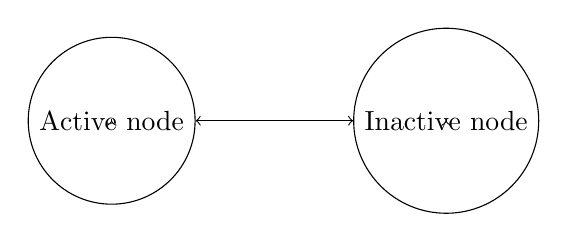
\begin{tikzpicture}[node distance=2cm]
        \node[draw, circle] (Active) {Active node};
        \node[draw, circle, right=of Active ] (Inactive) {Inactive node};

        \draw (Active) edge[->](Active);
        \draw (Active) edge[ ->](Inactive);
        \draw (Inactive) edge[ ->](Inactive);
        \draw (Inactive) edge[ ->](Active);
    \end{tikzpicture}
    \\
    \includegraphics[width=0.5\linewidth]{pregelprop.png}
\end{figure}

\subsection{Pregel API}
\subsubsection{Message passing}
A vertex can send any number of messages in a superstep. All messages sent to vertex V in superstep S are available. There is no guaranteed order of messages in the iterator, but it is guaranteed that messages will be delivered and that they will not be duplicated.

A vertex could learn the identifier of a non-neighbor from a message received earlier.

\subsubsection{Combiners}
Sending a message, especially to a vertex on another machine, incurs some overhead. This can be reduced in some cases with help from the user.  For example, suppose that Compute() receives integer messages and that only the sum
matters, as opposed to the individual values. In that case the system can combine several messages intended for a vertex V into a single message containing their sum, reducing the number of messages that must be transmitted and buffered.


\subsubsection{Aggregators}
Pregel aggregators are a mechanism for global communication,
monitoring, and data. Each vertex can provide a value
to an aggregator in superstep S, the system combines those
values using a reduction operator, and the resulting value
is made available to all vertices in superstep S + 1.

For instance, a sum
aggregator applied to the out-degree of each vertex yields the
total number of edges in the graph.

\subsubsection{Topology Mutations}
Just as a user’s Compute() function can send messages, it can also
issue requests to add or remove vertices or edges.

Additions follow removals, with vertex
addition before edge addition, and all mutations precede
calls to Compute(). This partial ordering yields deterministic
results for most conflicts. (compute -> remove -> addition)

\subsubsection{Input and output}
Users with unusual needs can write their own
by subclassing the abstract base classes Reader and Writer.

\subsection{Architecture}
\subsubsection{Partition}
The default partitioning function is just hash(ID)
mod N, where N is the number of partitions, but users can
replace it.

\subsubsection{Processing}
\begin{itemize}
    \item Many copies of the user program begin executing on
        a cluster of machines. One of these copies acts as the
        master. It is not assigned any portion of the graph, but
        is responsible for coordinating worker activity. The
        workers use the cluster management system’s name
        service to discover the master’s location, and send registration
        messages to the master.
    \item The master determines how many partitions the graph
        will have, and assigns one or more partitions to each
        worker machine. The number may be controlled by
        the user. Having more than one partition per worker
        allows parallelism among the partitions and better load
        balancing, and will usually improve performance. Each
        worker is responsible for maintaining the state of its
        section of the graph, executing the user’s Compute()
        method on its vertices, and managing messages to and
        from other workers. Each worker is given the complete
        set of assignments for all workers.
    \item The master assigns a portion of the user’s input to
        each worker. The input is treated as a set of records,
        each of which contains an arbitrary number of vertices
        and edges. The division of inputs is orthogonal to the
        partitioning of the graph itself, and is typically based
        on file boundaries. If a worker loads a vertex that belongs
        to that worker’s section of the graph, the appropriate
        data structures (Section 4.3) are immediately
        updated. Otherwise the worker enqueues a message to
        the remote peer that owns the vertex. After the input
        has finished loading, all vertices are marked as active.
    \item The master instructs each worker to perform a superstep.
        The worker loops through its active vertices, using
        one thread for each partition. The worker calls
        Compute() for each active vertex, delivering messages
        that were sent in the previous superstep. Messages are
        sent asynchronously, to enable overlapping of computation
        and communication and batching, but are delivered
        before the end of the superstep. When the worker
        is finished it responds to the master, telling the master
        how many vertices will be active in the next superstep.
        This step is repeated as long as any vertices are active,
        or any messages are in transit
    \item After the computation halts, the master may instruct
        each worker to save its portion of the graph.
\end{itemize}

\subsubsection{Fault tolerance}
Fault tolerance is achieved through checkpointing. At the
beginning of a superstep, the master instructs the workers
to save the state of their partitions to persistent storage,
including vertex values, edge values, and incoming messages;
the master separately saves the aggregator values.

If a worker does not receive a ping message after a specified interval, the worker
process terminates. If the master does not hear back from
a worker, the master marks that worker process as failed.
When one or more workers fail, the current state of the
partitions assigned to these workers is lost. The master reassigns
graph partitions to the currently available set of workers,
and they all reload their partition state from the most
recent available checkpoint at the beginning of a superstep S. 

\section{Summary : Resilient Distributed Datasets: A Fault-Tolerant Abstraction for In-Memory Cluster Computing}

The paper proposes a new abstraction called resilient
distributed datasets (RDDs) that enables efficient
data reuse in a broad range of applications. RDDs are
fault-tolerant, parallel data structures that let users explicitly
persist intermediate results in memory, control
their partitioning to optimize data placement, and manipulate
them using a rich set of operators.
The main challenge in designing RDDs is defining a
programming interface that can provide fault tolerance
efficiently.

\subsection{RDDs}

Formally, an RDD is a read-only, partitioned collection
of records. RDDs can only be created through deterministic
operations on either (1) data in stable storage or (2)
other RDDs. We call these operations transformations to
differentiate them from other operations on RDDs. Examples
of transformations include map, filter, and join.

RDDs do not need to be materialized at all times. Instead,
an RDD has enough information about how it was
derived from other datasets (its lineage) to compute its
partitions from data in stable storage. This is a powerful
property: in essence, a program cannot reference an
RDD that it cannot reconstruct after a failure.

users can control two other aspects of RDDs:
persistence and partitioning. Users can indicate which
RDDs they will reuse and choose a storage strategy for
them (e.g., in-memory storage). They can also ask that
an RDD’s elements be partitioned across machines based
on a key in each record. This is useful for placement optimizations,
such as ensuring that two datasets that will
be joined together are hash-partitioned in the same way.

\subsection{Spark Programming Interface}

Spark is an implementation of RDDs.

\subsection{Advantages of the RDD Model}

\begin{tabular}{l|p{5cm}|p{5cm}}
\textbf{Aspect} & \textbf{RDDs} & \textbf{Distributed Memory (DSM)} \\
\hline
\hline
Reads & Coarse- or fine-grained & Fine-grained \\ \hline
Writes & Coarse-grained & Fine-grained  \\ \hline
Consistency & Trivial (immutable)  & Up to app / runtime \\ \hline
Fault recovery & Fine-grained and lowoverhead using lineage & Requires checkpoints and program rollback \\ \hline
Straggler mitigation & Possible using backup tasks & Difficult \\ \hline
Work placement & Automatic based on data locality & Up to app (runtimes aim for transparency) \\ \hline
Behavior if not enough RAM & Similar to existing data flow systems & Poor performance (swapping?) \\ \hline
\end{tabular}

\subsection{Applications Not Suitable for RDDs}
RDDs are best suited for batch applications that apply the same operation to
all elements of a dataset. In these cases, RDDs can ef-
ficiently remember each transformation as one step in a
lineage graph and can recover lost partitions without having
to log large amounts of data. RDDs would be less
suitable for applications that make asynchronous finegrained
updates to shared state, such as a storage system
for a web application or an incremental web crawler.

\subsection{Application suitable for RDDs}
Iterative Machine Learning Applications. Page rank with optimized partitioning of the RDDs. In-Memory Analytics. Traffic Modeling. Twitter Spam Classification.


\subsection{Checkpointing}

Although lineage can always be used to recover RDDs
after a failure, such recovery may be time-consuming for
RDDs with long lineage chains. Thus, it can be helpful
to checkpoint some RDDs to stable storage.

\subsection{Memory Management}
Three options : Memory, serealized in memory, hard-drive.

\subsection{Expressing MapReduce with Spark}
MapReduce can be expressed using the
flatMap and groupByKey operations in Spark, or reduceByKey
if there is a combiner.

\section{Summary Towards Predictable Datacenter Networks}

Since tenants pay based on the time they occupy their
VMs, and this time is influenced by the network, tenants
implicitly end up paying for the network traffic; yet, such
communication is supposedly free (hidden cost).

\subsection{Virtual Network Abstractions}

The “virtual” nature of the network implies that the provider
has a lot of freedom in terms of the topology of this
network, and can offer different options to tenants for different
costs. Beyond the overarching goal of maintaining the
simplicity of the interface between tenants and providers,
our topologies or virtual network abstractions are guided by
two design goals:

\begin{description}
\item[Tenant suitability] The abstractions should allow tenants
to reason in an intuitive way about the network performance
of their applications when running atop the virtual
network.
\item[Provider flexibility] Providers should be able to multiplex
many virtual networks on their physical network.
The greater the amount of sharing possible, the lesser
the tenant costs.
\end{description}

To this effect, we propose two novel abstractions for virtual
networks in the following sections.

\subsubsection{Virtual Cluster}

\includegraphics[width=0.8\linewidth]{img/virt_switch.png}

With a virtual cluster, a tenant request
<N, B> provides the following topology: each tenant
machine is connected to a virtual switch by a bidirectional
link of capacity B, resulting in a one-level tree topology. The
virtual switch has a bandwidth of $N \times B$. This ensures that
the virtual network has no oversubscription and the maximum
rate at which the tenant VMs can exchange data is
N ∗ B. However, this data rate is only feasible if the communication
matrix for the tenant application ensures that each VM sends and receives at rate B. Alternatively, if all N
tenant VMs were to send data to a single destination VM,
the data rate achieved will be limited to B.
Since a virtual cluster offers tenants a network with no
oversubscription, \textbf{it is suitable for data-intensive applications
like MapReduce and BLAST}. For precisely such applications,
Amazon’s Cluster Compute provides tenants with
compute instances connected through a dedicated 10 Gbps
network with no oversubscription. This may be regarded as
a specific realization of the virtual cluster abstraction with
<N , 10 Gbps>.

\subsubsection{Virtual Oversubscribed Cluster}

\includegraphics[width=0.8\linewidth]{img/virt_over_subscribed.png}

While a network with no oversubscription is imperative
for data-intensive applications, this does not hold for many
other applications [19,34]. Instead, a lot of cloud bound applications
are structured in the form of components with
more intra-component communication than inter-component
communication [16,25]. A “Virtual Oversubscribed Cluster”
is better suited for such cases; it capitalizes on application
structure to reduce the bandwidth needed from the underlying
physical infrastructure compared to virtual clusters,
thereby improving provider flexibility and reducing tenant
costs.

With a virtual oversubscribed cluster, a tenant request
<N , B, S, O>. Tenant
machines are arranged in groups of size S, resulting in $\frac{n}{s}$ groups. VMs in a group are connected by bidirectional links
of capacity $B$ to a (virtual) group switch. The group switches
are further connected using a link of capacity $B' = \frac{S \times B}{O}$ 
to a (virtual) root switch. The resulting topology has no oversubscription
for intra-group communication. However, intergroup
communication has an oversubscription factor $O$, i.e.,
\textbf{the aggregate bandwidth at the VMs is $O$ times greater than
the bandwidth at the root switch}. Hence, this abstraction
closely follows the structure of typical oversubscribed datacenter
networks. Note, however, that $O$ neither depends upon
nor requires physical topology oversubscription. Compared to virtual cluster, this abstraction does not offer
as dense a connectivity. However, the maximum data rate
with this topology is still $N \times B$.

The localized nature of the
tenant’s bandwidth demands resulting from this abstraction
allows the provider to fit more tenants on the physical network.
This, as our evaluation shows, has the potential to
significantly limit tenant costs. By incentivizing tenants to
expose the flexibility of their communication demands, the abstraction achieves better multiplexing which benefits both
tenants and providers. Amazon’s EC2 Spot Instances is
a good example of how tenants are willing to be flexible, especially
when it suits their application demands, if it means
lowered costs.

\includegraphics[width=0.7\linewidth]{img/net_comp.png}

\subsection{Oktopus}

With Oktopus,
tenants requesting VMs can opt for a (virtual) cluster or a
(virtual) oversubscribed cluster to connect their VMs.

 Two main components are used:

 \begin{description}
 \item[Management plane] A logically centralized network manager
(NM), upon receiving a tenant request, performs
admission control and maps the request to physical machines.
This process is the same as today’s setup except
that the NM needs to further account for network resources
and maintain bandwidth reservations across the
physical network.
\item[Data plane] Oktopus uses rate-limiting at endhost hypervisors
to enforce the bandwidth available at each VM.
This ensures that no explicit bandwidth reservations at
datacenter switches are required.
 \end{description}

 The network manager implements allocation algorithms
to allocate slots on physical machines to tenant requests in
an online fashion. For tenant requests involving a virtual
network, the NM needs to ensure that the corresponding
bandwidth demands can be met while maximizing the number
of concurrent tenants. To achieve this, the NM maintains
the following information :
\begin{itemize}
\item The datacenter network
topology
\item The residual bandwidth for each link in the
network
\item The empty slots on each physical machine
\item The allocation information for existing tenants,
including the physical machines they are allocated to, the
network routes between these machines and the bandwidth
reserved for the tenant at links along these routes
\end{itemize}

\subsection{End.}

See algorithm in the paper for allocation process, etc.


\section{Summary : In Search of an Understandable Consensus Algorithm}

\subsection{Replicated state machines}

\begin{center}
\includegraphics[scale=0.5]{img/repli_log}
\end{center}
\begin{itemize}
\item Consensus algorithm are used in the context of replicated state machines, used to solve a variety of fault tolerance problem in distributed systems.

\item Replicated state machines are typically implemented using a replicated log, as shown in Figure 1. Each server stores a log containing a series of commands, which its state machine executes in order. Each log contains the same commands in the same order, so each state ma- chine processes the same sequence of commands. Since the state machines are deterministic, each computes the same state and the same sequence of outputs.

\item Keeping the replicated log consistent is the job of the consensus algorithm. It ensures that every log will eventually contains the same requests in the same order. Each server's state machine processes the requests in log order and the outputs are returned to clients. The servers appear to form a single, highly reliable state machine. 

\item Consensus algorithms have the following properties :
\begin{itemize}
\item Safety : never return an incorrect result
\item Available : fully functional as long as a majority of the servers are operational and can communicate with each other and with clients.
\item Consistency : they don't depend on timing to ensure the consistency of the logs.
\item A command can complete as soon as a majority of the cluster has responded to a single round of remote procedure calls.
\end{itemize}

\end{itemize}

\subsection{Drawbacks of Paxos}

\begin{enumerate}
\item Difficult to understand.
\item Paxos doesn't provide a good foundation for building practical implementation.
\begin{itemize}
\item No widely agreed-upon algorithm for multi-Paxos (Combination of of multiple instances of single-decree Paxos to facilitate a series of decisions such as a log).
\item Paxos architecture is a poor one of building practical systems. This is a consequence of the single-decree decomposition.
\item Paxos uses a symmetric peer-to-peer approach as its core. This is not practical for system that need to made several decisions. It would be simpler and faster to first select a leader and then have the leader coordinates the decisions. 
\end{itemize}
\end{enumerate}

\subsection{Raft consensus algorithm}

\subsubsection{Basics}
\begin{itemize}

\item At any given time, each server is one of the three states : \textit{leader, follower, candidate}; 
\begin{itemize}
\item \textbf{Followers }: they issue no request on their own but simply respond to requests from leaders and candidates.
\item \textbf{Leader : } it handles all client requests.
\item \textbf{Candidate : } this state is used to elect a new leader.
\end{itemize}


\item Raft divides time into terms of arbitrary length. Each term begins with an election in order to have a new leader. If the election results in a split vote, there is no leader for this term and a new term with a new election will start shortly after. The terms act as logical clock, they allow servers to detect obsolete information. Each server stores a current term number. If one server's term is smaller then the other's then it updates its current term to the larger value. If a leader or a candidate discovers that its term is out of date, it immediately reverts to follower state. If a server receives a request with a stale term number, it rejects the request. Current term are exchanged when servers communicate with each other. 

\item Servers communicate with each other thanks to remote procedure calls. Especially, the \textbf{request vote} RPCs and the \textbf{append entries} RPCs. The first is initiated by candidates during the election and the second one by leader to replicate log entries and to provide a form of heartbeat. 

\end{itemize}

\subsubsection{Leader election}

\begin{itemize}

\item A server remains in the follower state as long as it receives heartbeat from the leader. If a follower receives no communication over the election timeout, it assumes there is no viable leader and begins an election. The election mechanism is the following :
\begin{enumerate}
\item A follower (the one who didn't receive heartbeat) increments its current term and transitions to candidate state. It then votes for itself and issues a \textbf{request vote} RPCs to the other servers.
\item Each server vote for at most one candidate in a given term, on a first-come-first-served basis. This can lead to two situations :
\begin{enumerate}
\item A candidate wins the election by receiving vote from a majority of servers. It then sends heartbeat to establish its authority.
\item Splite vote, and no leader for this term.
\end{enumerate}

\item To insure that the split vote situation doesn't happen again and again, Raft uses randomized election timeouts. Each candidate restarts its election timeout at the start of the election and it waits for that amount of time before starting the next election. By making this time random, the split vote situation is unlikely to happen often.
\end{enumerate}
\end{itemize}
\subsubsection{Log replication}

\begin{center}
\includegraphics[scale=0.5]{img/logs}
\end{center}

\begin{itemize}


\item When communicating with the leader, clients send request with command to be executed by the replicated state machine. The leader appends the command to its log as a new entry and issued an \textbf{AppendEntries} RPCs to each servers to replicate the entry. The leader retries \textbf{AppendEntries} RPCs indefinitely until all followers eventually store all log entries, and applies the entry to its state machine and returns the result to the client. Raft guarantees that applied entries are durable and will eventually be executed by all of the available state machines. An entry is applied (committed) once the leader has replicated it on a majority of the servers. 


\item Log organization is shown on the figure. Each log entry has an integer to identify its position in the log and an integer with the term number when the entry was received. If two entries in different logs have the same index and term, then they store the same command and the logs are identical in all preceding entries. 

\item When issuing a \textbf{AppendEntries} for a new entry, the leader includes the index and term of the entry that precedes the new entry. If the follower doesn't find an entry in its log with the same index and term, it refuses the new entry and warns the leader that the entry was rejected. The leader maintains a \textit{nextIndex} for each follower which is the index of the next log entry the leader will send to that follower. When it receives a rejection, the leader decrements \textit{nextIndex} and retries the AppendEntries and such until the entry is accepted by the follower. Once the entry is accepted, the leader knows that the follower has the same log than its own ending at \textit{nextIndex}. It then forces the follower's log to duplicate its own starting at \textit{nextIndex}.

\end{itemize}

\subsubsection{Safety}

\paragraph*{Election restriction}
In order to ensure that the leader for any given term contains all of the entries committed in previous terms, Raft adds a restriction on which servers may be elected leader. Raft uses the voting process to prevent a candidate from winning an election unless its log contains all committed entries. If the candidate's log is at least as up-to-date as any other log in the majority, then if will hold all the committed entries and can be elected as leader. The \textbf{RequestVote} RPCs implements this restriction by including information about the candidate's log and the voter denies its vote if its own log is more up-to-date than that of the candidate. 

\paragraph{Timing and availability}
Leader election is the aspect of Raft where timing is most critical. Raft will be able to elect and maintain a steady leader as long as the system satisfies the following timing requirement : Broadcast Time $<<$ election Timeout $<<$ MTBF. Broadcast time is the average time for a server to send RPCs to every server in the cluster and receive their response; MTBF is the average time between failures for a single server. The broadcast time should be smaller than the election timeout so that leaders can reliably send the heartbeat to keep followers from starting elections. The election timeout should be less than MTBF so that the system makes steady progress. 

\subsection{Custer Membership changes}

In practice, it will be necessary to change the configuration (replace server, change degree of replication,...). Raft handles configuration changes without having to take the entire cluster off-line. To be safe, there must be no point during the transition where two leader can be elected for the same term. In order to achieve that goal, configuration changes must use a two-phase approach. First phase switches to a transitional configuration called joint consensus. Once the joint consensus has been committed, the system transitions to the new configuration. The joint consensus combines both the old and the new configuration : 
\begin{itemize}
\item All the log entries are replicated to all servers in both configuration
\item Any server from either configuration may serve as leader
\item Agreement requires separate majorities from \textit{both} the old and new configuration. 
\end{itemize}

Three more issues are still possible :

\begin{enumerate}
\item New servers in the configuration may not initially store any log entries (since they are new ones). The new servers join the cluster as non-voting members. The leader replicates log entries to them but they are not considered for majorities.
\item The cluster leader may not be part of the new configuration. The leader returns to the follower state once it has committed the log entries for the new configuration. There is then a time when the leader is managing a cluster that does not include itself; it replicates log entries but is not taken into account for majorities. 
\item Removed servers can disrupt the cluster. These servers will not re- ceive heartbeats, so they will time out and start new elec- tions. They will then send RequestVote RPCs with new term numbers, and this will cause the current leader to revert to follower state. A new leader will eventually be elected, but the removed servers will time out again and the process will repeat, resulting in poor availability. To prevent this problem, servers disregard RequestVote RPCs when they believe a current leader exists. This does not affect normal elections, where each server waits at least a minimum election timeout before starting an election. However, it helps avoid disruptions from re- moved servers: if a leader is able to get heartbeats to its cluster, then it will not be deposed by larger term numbers.
\end{enumerate}


\section{ZooKeeper: Wait-free coordination for Internet-scale systems}
This section might be redundant with what has been said in the course, nevertheless, it gives a quick view of what the document is about.

Zookeeper is a service for coordinating processes of distributed applications. The core design principle of Zookeeper is to not implement services for each different coordination needs (called primitives) but instead to it exposes an API that enable the development of such primitives. This lead to the implementation of a \textbf{coordination kernel} that enables new primitives without requiring changes to the service core.

\subsection{Zookeeper service}

Before going further a little terminology might be of use:
\begin{itemize}
\item \textbf{Client}: user of Zookeeper service.
\item \textbf{Server}: process providing the Zookeper service.
\item \textbf{Znode}: in-memory data node in the Zookeeper data.
\item \textbf{Session}: a client connects to Zookeeper and initiates a session. The session ends when the client explicitly close a session handle or Zookeeper detects the client as faulty (through a session-timeout $\Leftrightarrow$ the client hasn't send anything for a given time)
\end{itemize}

Znodes can be further divided : 

\begin{itemize}
	\item \textbf{regular}: clients manipulate regular znodes by creating and deleting them explicitly.
	\item \textbf{ephemeral}: clients can delete them explicitly or let the system remove them automatically when their session terminates.
\end{itemize}

\begin{figure}
	\begin{center}
		\includegraphics[scale=1]{img/hierachicalZookeeper.png}
	\end{center}
	\caption{Illustration of ZooKeeper hierarchical name space}
	\label{hierarchicalname}
\end{figure}

Znodes are organized according to a hierarchical name space. It is roughly the same as for a file system, see figure \ref{hierarchicalname}. The nodes in this hierarchy are data objects that clients manipulate through the ZooKeeper API. All znodes store data, and all znodes, except for ephemeral znodes, can have children.

When creating a new znode, a client can set the \textbf{sequential flag}: Nodes created with this flag set have the value of a monotonically increasing counter appended to its name.

When a client wants to have notifications of changes done on some data. This is done through watches, when the client issues a read operation, the operation completes as normal but the server promises to notify the client when the information returned has changes. Watches are one-time trigger.



\subsection{Guarantees}
Zookeeper has two basic ordering guarantees: 
\begin{itemize}
\item \textbf{Linearizable writes}: all requests that update the state of Zookeeper are serializable and respect precedence. This is assured through the leader-based atomic broadcast protocol called Zab
\item \textbf{FIFO client order}: all requests from a given client are executed in the order that the were sent by the client.
\end{itemize}

The paper also focuses on some problem that can arise in certain circumstances, go and see section 2.3 of the document (it is done with an example).

Zookeeper adds two other guarantees:
\begin{itemize}
\item \textbf{liveness}: if a majority of Zookeeper servers are active and communicating the service will be available
\item \textbf{durability}: if ZooKeeper responds successfully to a change request, that change persists across any number of failures as long a a quorum of servers ($\approx$ majority) is eventually able to recover.
\end{itemize}

The paper also focuses on examples of primitives implementations see section 2.4.
\subsection{Zookeeper Implementation}

When a client sends a write request, it is forwarded to a single server called the leader The rest of the ZooKeeper servers, called followers, receive message proposals consisting of state changes from the leader and agree upon state changes. In fact the leader executes the request and then broadcast the change to the ZooKeeper state through Zab, an atomic broadcast protocol.

Going from the request of the client to the changes of the ZooKeeper state is done using transactions. When a leader receives a write request, it calculates what the state of the system will be when the write is applied and transforms it into a transaction that captures this new state.

Transactions are idempotent, meaning that applying this transaction one or several times won't make any difference.


\end{document}
